% Seminar 5: Conditional volatility: ARCH and GARCH
% Time Series Analysis -- Bachelor's programmes Economic Informatics and Economic Cybernetics, Bucharest University of Economic Studies
% GENERATED by latex/build_seminar5.py -- edit the generator, not this file.
% Student version by default; the instructor version is the *_solutions.tex wrapper.
\makeatletter\@ifundefined{ifsolutions}{\expandafter\newif\csname ifsolutions\endcsname}{}\makeatother

\newcommand{\coursename}{Time Series Analysis}
% Preambul comun TSA -- Serii de timp / Time Series Analysis (Beamer, 16:9)
% Același design ca MFM și SFM (preluat din SFM, 5 octombrie 2026). Înainte de % Preambul comun TSA -- Serii de timp / Time Series Analysis (Beamer, 16:9)
% Același design ca MFM și SFM (preluat din SFM, 5 octombrie 2026). Înainte de % Preambul comun TSA -- Serii de timp / Time Series Analysis (Beamer, 16:9)
% Același design ca MFM și SFM (preluat din SFM, 5 octombrie 2026). Înainte de \input{../../latex/preamble} se definește
%   \newcommand{\coursename}{Time Series Analysis}      (EN)
%   \newcommand{\coursename}{Serii de timp}       (RO)  și  \def\tsalang{ro}
% Fișierele .tex se află în EN/Courses, EN/Seminars, RO/Cursuri, RO/Seminarii (două niveluri sub rădăcină).
% Deck-urile sînt generate de latex/build_chapterN.py / build_seminarN.py (vezi latex/tsa_build.py).

\documentclass[9pt, aspectratio=169, t]{beamer}
\providecommand{\coursename}{Time Series Analysis}

% Ensure content fits on slides
\setbeamersize{text margin left=8mm, text margin right=8mm}
% Smaller institute font (title page)
\setbeamerfont{institute}{size=\footnotesize}

%=============================================================================
% THEME AND STYLE CONFIGURATION
%=============================================================================
\usetheme{default}
% Using default theme for clean header/footer control

% Color Palette (matching Redispatch PDF)
\definecolor{MainBlue}{RGB}{26, 58, 110}
\definecolor{AccentBlue}{RGB}{26, 58, 110}
\definecolor{IDAred}{RGB}{205, 0, 0}
\definecolor{DarkGray}{RGB}{51, 51, 51}
\definecolor{MediumGray}{RGB}{128, 128, 128}
\definecolor{LightGray}{RGB}{248, 248, 248}
\definecolor{VeryLightGray}{RGB}{235, 235, 235}
\definecolor{KeynoteGray}{RGB}{218, 218, 218}
\definecolor{SectionGray}{RGB}{120, 120, 120}
\definecolor{FooterGray}{RGB}{100, 100, 100}
\definecolor{Crimson}{RGB}{220, 53, 69}
\definecolor{Forest}{RGB}{46, 125, 50}
\definecolor{Amber}{RGB}{181, 133, 63}
\definecolor{Orange}{RGB}{230, 126, 34}
\definecolor{Purple}{RGB}{142, 68, 173}

% Gradient background (exact Keynote 315° gradient: white to RGB 218,218,218)
\setbeamertemplate{background}{%
    \begin{tikzpicture}[remember picture, overlay]
        \shade[shading=axis, shading angle=315,
        top color=white, bottom color=KeynoteGray]
        (current page.south west) rectangle (current page.north east);
    \end{tikzpicture}%
}
% Fallback solid color for compatibility
\setbeamercolor{background canvas}{bg=}

\setbeamercolor{palette primary}{bg=MainBlue, fg=white}
\setbeamercolor{palette secondary}{bg=MainBlue!85, fg=white}
\setbeamercolor{palette tertiary}{bg=MainBlue!70, fg=white}
\setbeamercolor{structure}{fg=MainBlue}
\setbeamercolor{title}{fg=IDAred}
\setbeamercolor{frametitle}{fg=IDAred, bg=}
\setbeamercolor{block title}{bg=MainBlue, fg=white}
\setbeamercolor{block body}{bg=VeryLightGray, fg=DarkGray}
\setbeamercolor{block title alerted}{bg=Crimson, fg=white}
\setbeamercolor{block body alerted}{bg=Crimson!8, fg=DarkGray}
\setbeamercolor{block title example}{bg=Forest, fg=white}
\setbeamercolor{block body example}{bg=Forest!8, fg=DarkGray}
\setbeamercolor{item}{fg=MainBlue}

% Footer colors (override Madrid theme blue)
\setbeamercolor{author in head/foot}{fg=FooterGray, bg=}
\setbeamercolor{title in head/foot}{fg=FooterGray, bg=}
\setbeamercolor{date in head/foot}{fg=FooterGray, bg=}
\setbeamercolor{section in head/foot}{fg=FooterGray, bg=}
\setbeamercolor{subsection in head/foot}{fg=FooterGray, bg=}

% Bullet styles (apply everywhere including blocks)
\setbeamertemplate{itemize item}{\color{MainBlue}$\boxdot$}
\setbeamertemplate{itemize subitem}{\color{MainBlue}$\blacktriangleright$}
\setbeamertemplate{itemize subsubitem}{\color{MainBlue}\tiny$\bullet$}
\setbeamertemplate{itemize/enumerate body begin}{\normalsize}
\setbeamertemplate{itemize/enumerate subbody begin}{\normalsize}

% Item spacing - compact style
\setlength{\leftmargini}{10pt}       % Level 1: minimal indent
\setlength{\leftmarginii}{10pt}      % Level 2: minimal additional indent
% Compact list spacing (zero extra space before/after lists in blocks)
\makeatletter
\def\@listi{\leftmargin\leftmargini \topsep 0pt \parsep 0pt \itemsep 0pt}
\def\@listii{\leftmargin\leftmarginii \topsep 0pt \parsep 0pt \itemsep 0pt}
\makeatother

\setbeamertemplate{navigation symbols}{}

%=============================================================================
% CUSTOM HEADLINE
%=============================================================================
\setbeamertemplate{headline}{%
    \vskip10pt%
    \hbox to \paperwidth{%
        \hskip0.5cm%
        {\small\color{FooterGray}\renewcommand{\hyperlink}[2]{##2}\insertsectionhead}%
        \hfill%
        \textcolor{FooterGray}{\small\insertframenumber}%
        \hskip0.5cm%
    }%
    \vskip4pt%
    {\color{FooterGray}\hrule height 0.4pt}%
}

%=============================================================================
% CUSTOM FOOTER
%=============================================================================
\usepackage{fontawesome5}

\setbeamertemplate{footline}{%
    {\color{FooterGray}\hrule height 0.4pt}%
    \vskip4pt%
    \hbox to \paperwidth{%
        \hskip0.5cm%
        \textcolor{FooterGray}{\small\coursename}%
        \hfill%
        \raisebox{-0.1em}{%
            \begin{tikzpicture}[x=0.08em, y=0.08em, line width=0.4pt]
                \draw[FooterGray] (0,3) -- (1,4) -- (2,3.5) -- (3,5) -- (4,4) -- (5,6) -- (6,5.5) -- (7,4) -- (8,5) -- (9,7) -- (10,6) -- (11,5) -- (12,6.5) -- (13,8) -- (14,7) -- (15,6) -- (16,7.5) -- (17,9) -- (18,8) -- (19,7) -- (20,8.5) -- (21,10) -- (22,9) -- (23,8) -- (24,9.5);
            \end{tikzpicture}%
        }%
        \hskip0.5cm%
    }%
    \vskip6pt%
}

%=============================================================================
% PACKAGES
%=============================================================================
\usepackage[utf8]{inputenc}
\DeclareUnicodeCharacter{03B1}{\ensuremath{\alpha}}
\usepackage[T1]{fontenc}
\usepackage{amsmath, amssymb, amsthm}
\usepackage{mathtools}
\usepackage{bm}
\usepackage{tikz}
\usetikzlibrary{arrows.meta, positioning, shapes, calc, decorations.pathreplacing, shadings}
\usepackage{booktabs}
\usepackage{multirow}
\usepackage{array}
\usepackage{graphicx}
\usepackage{animate}
\usepackage{hyperref}
\usepackage{colortbl}
\usepackage{listings}
\lstset{language=Python, basicstyle=\ttfamily\scriptsize, keywordstyle=\color{MainBlue}\bfseries,
  commentstyle=\color{Forest}, stringstyle=\color{Crimson}, breaklines=true,
  frame=none, backgroundcolor=\color{VeryLightGray}, xleftmargin=2mm}
\hypersetup{colorlinks=true, linkcolor=MainBlue, urlcolor=MainBlue}
\graphicspath{{../../logos/}{../../charts/}{../../photos/}}
\usepackage{xcolor}
\hfuzz=2pt  % Suppress tiny overfull warnings (<2pt)
\vfuzz=2pt  % Suppress tiny vertical overfull warnings (<2pt)
% \mathrm in the sans-serif family of the slides (beamer resets \mathrm to the serif family at \begin{document};
% this hook runs after beamer's, so WN, Var, RMSE, ... in formulas match the surrounding text)
% Bold vectors and matrices in the same sans-serif family: \mathbf{A} in sans bold (beamer's own \mathbf came out in
% medium weight), and the bold upright Greek capitals of \boldsymbol / \bm (\bSigma, \bPhi, \boldsymbol{\Theta}) in
% cmss bold: bm.sty fixes its "boldoperators" font when it is loaded (serif cmbx), before beamer switches the
% operators to cmss, so it is reset here.
\AtBeginDocument{%
  \SetMathAlphabet{\mathrm}{normal}{\encodingdefault}{\sfdefault}{\mddefault}{n}%
  \SetMathAlphabet{\mathrm}{bold}{\encodingdefault}{\sfdefault}{bx}{n}%
  \SetMathAlphabet{\mathbf}{normal}{\encodingdefault}{\sfdefault}{bx}{n}%
  \SetMathAlphabet{\mathbf}{bold}{\encodingdefault}{\sfdefault}{bx}{n}%
  \SetSymbolFont{boldoperators}{normal}{OT1}{cmss}{bx}{n}%
  \SetSymbolFont{boldoperators}{bold}{OT1}{cmss}{bx}{n}}

%=============================================================================
% QUANTLET COMMANDS
%   \quantlet{<displayed name>}{<url>}       (generic, compatible with the older TSA decks)
%   \tsaquantlet{Ch_05}{TSA_ch5_garch}       -> https://github.com/danpele/Time-Series-Analysis/tree/main/Quantlets/Ch_05/TSA_ch5_garch
%   \qlurl{<folder>} is defined per chapter by the generator (Quantlets/Ch_NN/<folder>)
%=============================================================================
\newcommand{\tsarepo}{https://github.com/danpele/Time-Series-Analysis}
\newcommand{\tsaqlbase}{https://github.com/danpele/Time-Series-Analysis/tree/main/Quantlets}
\newcommand{\quantlet}[2]{%
    \hfill\href{#2}{%
        \raisebox{-0.15em}{
\includegraphics[height=0.7em]{ql_logo.png}}%
        \textcolor{MainBlue}{\tiny\ #1}%
    }%
}
\newcommand{\tsaquantlet}[2]{\quantlet{\detokenize{#2}}{\tsaqlbase/#1/#2}}

%=============================================================================
% NOTEBOOKS (Google Colab)
%   \colaburl{notebooks/EN/chapter5_seminar_notebook.ipynb} -> the Colab link of a file in the TSA repo
%   \nb: the chapter notebook (each seminar deck redefines it with \renewcommand)
%=============================================================================
\newcommand{\colaburl}[1]{https://colab.research.google.com/github/danpele/Time-Series-Analysis/blob/main/#1}
\newcommand{\nb}{https://colab.research.google.com/github/danpele/Time-Series-Analysis/tree/main/notebooks/EN}
\newcommand{\nbname}{notebooks/EN}

%=============================================================================
% SLIDE HELPERS (used by the generators; the same as in MFM)
%=============================================================================
% local font size for list bodies (the preamble forces \normalsize)
\newcommand{\itemsize}[1]{\setbeamertemplate{itemize/enumerate body begin}{#1}\setbeamertemplate{itemize/enumerate subbody begin}{#1}}
\newcommand{\intitle}[1]{{\hypersetup{urlcolor=white}#1}}   % white links inside coloured title bars
\newcommand{\imgcap}[1]{{\scriptsize #1}\\[0.5mm]}          % caption under a photo
\newcommand{\imgcredit}[2]{{\tiny\color{FooterGray}\href{#1}{#2}}}   % image credit: source URL, author/licence
\newcommand{\aiprompt}[1]{{\ttfamily\color{MainBlue}#1}}     % a prompt to an AI assistant

%=============================================================================
% SEMINARS: student version by default; the instructor wrapper *_solutions.tex sets \solutionstrue
%=============================================================================
\makeatletter\@ifundefined{ifsolutions}{\expandafter\newif\csname ifsolutions\endcsname}{}\makeatother
\newcommand{\solonly}[1]{\ifsolutions #1\fi}
\newcommand{\propsub}{\ifsolutions\else\framesubtitle{\ifdefined\tsalang Rezolvarea se discută la seminar\else Solution discussed in class\fi}\fi}

%=============================================================================
% APPENDIX AND CHAPTER LINKS (latex/appendix_links.py writes the calls; it also re-declares these
% macros before \begin{document}, so the decks compile with or without this preamble block)
%=============================================================================
\providecommand{\tsaapplink}[3]{\hypertarget{#2}{}\hyperlink{#1}{\beamergotobutton{#3}}}
\providecommand{\tsaappback}[2]{\begin{tikzpicture}[remember picture,overlay]\node[anchor=south east] at ([xshift=-3mm,yshift=7mm]current page.south east){\hyperlink{#1}{\beamerreturnbutton{#2}}};\end{tikzpicture}}
\providecommand{\tsachlink}[2]{\href{#1}{#2}}
\providecommand{\tsachlinkt}[2]{\href{#1}{\usebeamercolor[fg]{frametitle}#2}}

%=============================================================================
% QUANTINAR COMMAND: link către un curs Quantinar (subiecte avansate)
%=============================================================================
\newcommand{\quantinar}[2]{%
    \href{#2}{%
        \raisebox{-0.15em}{
\includegraphics[height=0.8em]{qr_logo.png}}%
        \textcolor{MainBlue}{\scriptsize\ #1}%
    }%
}

%=============================================================================
% CUSTOM TITLE PAGE
%=============================================================================
\defbeamertemplate*{title page}{hybrid}[1][]
{
    \vspace{0.2cm}
    % Logos row - top header (with clickable links)
    \begin{center}
        \href{https://www.ase.ro}{
\includegraphics[height=1.0cm]{ase_logo.png}}\hspace{0.3cm}%
        \href{https://theida.net}{
\includegraphics[height=1.0cm]{ida_logo.png}}\hspace{0.3cm}%
        \href{https://blockchain-research-center.com}{
\includegraphics[height=1.0cm]{brc_logo.png}}\hspace{0.3cm}%
        \href{https://www.ai4efin.ase.ro}{
\includegraphics[height=1.0cm]{ai4efin_logo.png}}\hspace{0.3cm}%
        \href{https://ipe.ro/new}{
\includegraphics[height=1.0cm]{acad_logo.png}}\hspace{0.3cm}%
        \href{https://www.digital-finance-msca.com}{
\includegraphics[height=1.0cm]{msca_logo.png}}%
    \end{center}

    \vspace{0.6cm}

    % Main title with Q logos on sides (with clickable links)
    \begin{center}
        \begin{minipage}{0.1\textwidth}
            \centering
            \href{https://quantlet.com}{
\includegraphics[height=1.1cm]{ql_logo.png}}
        \end{minipage}%
        \begin{minipage}{0.78\textwidth}
            \centering
            {\LARGE\bfseries\usebeamercolor[fg]{title}\inserttitle}

            \vspace{0.3cm}

            {\usebeamerfont{subtitle}\usebeamercolor[fg]{title}\insertsubtitle}
        \end{minipage}%
        \begin{minipage}{0.1\textwidth}
            \centering
            \href{https://quantinar.com}{
\includegraphics[height=1.1cm]{qr_logo.png}}
        \end{minipage}
    \end{center}

    \vspace{0.6cm}

    % Authors (left aligned)
    \hspace{0.5cm}{\usebeamerfont{author}\insertauthor}

    \vspace{0.3cm}

    % Institute/Affiliations (left aligned)
    \hspace{0.5cm}\begin{minipage}[t]{0.9\textwidth}
        \raggedright\small\insertinstitute
    \end{minipage}
}

%=============================================================================
% THEOREM ENVIRONMENTS
%=============================================================================
\theoremstyle{definition}
\setbeamertemplate{theorems}[numbered]
\ifdefined\tsalang
\newtheorem{defn}{Definiție}
\newtheorem{thm}{Teoremă}
\newtheorem{prop}{Propoziție}
\newtheorem{rmk}{Observație}
\else
\newtheorem{defn}{Definition}
\newtheorem{thm}{Theorem}
\newtheorem{prop}{Proposition}
\newtheorem{rmk}{Remark}
\fi

%=============================================================================
% CENTRED MINIPAGE (no extra vertical space)
%=============================================================================
\newenvironment{cminipage}[1]{%
    \par\noindent\hfill\begin{minipage}{#1}\ignorespaces
}{%
    \end{minipage}\hfill\null\par
}

%=============================================================================
% CUSTOM COMMANDS
%=============================================================================
\newcommand{\E}{\mathbb{E}}
\newcommand{\Var}{\text{Var}}
\newcommand{\Cov}{\text{Cov}}
\newcommand{\Corr}{\text{Corr}}
\newcommand{\R}{\mathbb{R}}
\newcommand{\N}{\mathbb{N}}
\newcommand{\Z}{\mathbb{Z}}
\newcommand{\B}{\mathbf{B}}
\newcommand{\imark}{\textcolor{MainBlue}{\textbullet}}
\newcommand{\RMSE}{\text{RMSE}}
\newcommand{\MAE}{\text{MAE}}
\newcommand{\MAPE}{\text{MAPE}}

% Boldface vector/matrix commands (VAR, VECM, state space; also used by the older TSA decks)
\newcommand{\bY}{\mathbf{Y}}
\newcommand{\bX}{\mathbf{X}}
\newcommand{\bA}{\mathbf{A}}
\newcommand{\bB}{\mathbf{B}}
\newcommand{\bepsilon}{\boldsymbol{\varepsilon}}
\newcommand{\bSigma}{\boldsymbol{\Sigma}}
\newcommand{\bPhi}{\boldsymbol{\Phi}}
\newcommand{\bGamma}{\boldsymbol{\Gamma}}
\newcommand{\bPi}{\boldsymbol{\Pi}}
\newcommand{\bc}{\mathbf{c}}
\newcommand{\balpha}{\boldsymbol{\alpha}}
\newcommand{\bbeta}{\boldsymbol{\beta}}
\newcommand{\bvarepsilon}{\boldsymbol{\varepsilon}}

% Legacy seminar marks (older TSA seminar decks)
\newcommand{\correct}{\textcolor{Forest}{\checkmark}}
\newcommand{\incorrect}{\textcolor{Crimson}{\texttimes}}
 se definește
%   \newcommand{\coursename}{Time Series Analysis}      (EN)
%   \newcommand{\coursename}{Serii de timp}       (RO)  și  \def\tsalang{ro}
% Fișierele .tex se află în EN/Courses, EN/Seminars, RO/Cursuri, RO/Seminarii (două niveluri sub rădăcină).
% Deck-urile sînt generate de latex/build_chapterN.py / build_seminarN.py (vezi latex/tsa_build.py).

\documentclass[9pt, aspectratio=169, t]{beamer}
\providecommand{\coursename}{Time Series Analysis}

% Ensure content fits on slides
\setbeamersize{text margin left=8mm, text margin right=8mm}
% Smaller institute font (title page)
\setbeamerfont{institute}{size=\footnotesize}

%=============================================================================
% THEME AND STYLE CONFIGURATION
%=============================================================================
\usetheme{default}
% Using default theme for clean header/footer control

% Color Palette (matching Redispatch PDF)
\definecolor{MainBlue}{RGB}{26, 58, 110}
\definecolor{AccentBlue}{RGB}{26, 58, 110}
\definecolor{IDAred}{RGB}{205, 0, 0}
\definecolor{DarkGray}{RGB}{51, 51, 51}
\definecolor{MediumGray}{RGB}{128, 128, 128}
\definecolor{LightGray}{RGB}{248, 248, 248}
\definecolor{VeryLightGray}{RGB}{235, 235, 235}
\definecolor{KeynoteGray}{RGB}{218, 218, 218}
\definecolor{SectionGray}{RGB}{120, 120, 120}
\definecolor{FooterGray}{RGB}{100, 100, 100}
\definecolor{Crimson}{RGB}{220, 53, 69}
\definecolor{Forest}{RGB}{46, 125, 50}
\definecolor{Amber}{RGB}{181, 133, 63}
\definecolor{Orange}{RGB}{230, 126, 34}
\definecolor{Purple}{RGB}{142, 68, 173}

% Gradient background (exact Keynote 315° gradient: white to RGB 218,218,218)
\setbeamertemplate{background}{%
    \begin{tikzpicture}[remember picture, overlay]
        \shade[shading=axis, shading angle=315,
        top color=white, bottom color=KeynoteGray]
        (current page.south west) rectangle (current page.north east);
    \end{tikzpicture}%
}
% Fallback solid color for compatibility
\setbeamercolor{background canvas}{bg=}

\setbeamercolor{palette primary}{bg=MainBlue, fg=white}
\setbeamercolor{palette secondary}{bg=MainBlue!85, fg=white}
\setbeamercolor{palette tertiary}{bg=MainBlue!70, fg=white}
\setbeamercolor{structure}{fg=MainBlue}
\setbeamercolor{title}{fg=IDAred}
\setbeamercolor{frametitle}{fg=IDAred, bg=}
\setbeamercolor{block title}{bg=MainBlue, fg=white}
\setbeamercolor{block body}{bg=VeryLightGray, fg=DarkGray}
\setbeamercolor{block title alerted}{bg=Crimson, fg=white}
\setbeamercolor{block body alerted}{bg=Crimson!8, fg=DarkGray}
\setbeamercolor{block title example}{bg=Forest, fg=white}
\setbeamercolor{block body example}{bg=Forest!8, fg=DarkGray}
\setbeamercolor{item}{fg=MainBlue}

% Footer colors (override Madrid theme blue)
\setbeamercolor{author in head/foot}{fg=FooterGray, bg=}
\setbeamercolor{title in head/foot}{fg=FooterGray, bg=}
\setbeamercolor{date in head/foot}{fg=FooterGray, bg=}
\setbeamercolor{section in head/foot}{fg=FooterGray, bg=}
\setbeamercolor{subsection in head/foot}{fg=FooterGray, bg=}

% Bullet styles (apply everywhere including blocks)
\setbeamertemplate{itemize item}{\color{MainBlue}$\boxdot$}
\setbeamertemplate{itemize subitem}{\color{MainBlue}$\blacktriangleright$}
\setbeamertemplate{itemize subsubitem}{\color{MainBlue}\tiny$\bullet$}
\setbeamertemplate{itemize/enumerate body begin}{\normalsize}
\setbeamertemplate{itemize/enumerate subbody begin}{\normalsize}

% Item spacing - compact style
\setlength{\leftmargini}{10pt}       % Level 1: minimal indent
\setlength{\leftmarginii}{10pt}      % Level 2: minimal additional indent
% Compact list spacing (zero extra space before/after lists in blocks)
\makeatletter
\def\@listi{\leftmargin\leftmargini \topsep 0pt \parsep 0pt \itemsep 0pt}
\def\@listii{\leftmargin\leftmarginii \topsep 0pt \parsep 0pt \itemsep 0pt}
\makeatother

\setbeamertemplate{navigation symbols}{}

%=============================================================================
% CUSTOM HEADLINE
%=============================================================================
\setbeamertemplate{headline}{%
    \vskip10pt%
    \hbox to \paperwidth{%
        \hskip0.5cm%
        {\small\color{FooterGray}\renewcommand{\hyperlink}[2]{##2}\insertsectionhead}%
        \hfill%
        \textcolor{FooterGray}{\small\insertframenumber}%
        \hskip0.5cm%
    }%
    \vskip4pt%
    {\color{FooterGray}\hrule height 0.4pt}%
}

%=============================================================================
% CUSTOM FOOTER
%=============================================================================
\usepackage{fontawesome5}

\setbeamertemplate{footline}{%
    {\color{FooterGray}\hrule height 0.4pt}%
    \vskip4pt%
    \hbox to \paperwidth{%
        \hskip0.5cm%
        \textcolor{FooterGray}{\small\coursename}%
        \hfill%
        \raisebox{-0.1em}{%
            \begin{tikzpicture}[x=0.08em, y=0.08em, line width=0.4pt]
                \draw[FooterGray] (0,3) -- (1,4) -- (2,3.5) -- (3,5) -- (4,4) -- (5,6) -- (6,5.5) -- (7,4) -- (8,5) -- (9,7) -- (10,6) -- (11,5) -- (12,6.5) -- (13,8) -- (14,7) -- (15,6) -- (16,7.5) -- (17,9) -- (18,8) -- (19,7) -- (20,8.5) -- (21,10) -- (22,9) -- (23,8) -- (24,9.5);
            \end{tikzpicture}%
        }%
        \hskip0.5cm%
    }%
    \vskip6pt%
}

%=============================================================================
% PACKAGES
%=============================================================================
\usepackage[utf8]{inputenc}
\DeclareUnicodeCharacter{03B1}{\ensuremath{\alpha}}
\usepackage[T1]{fontenc}
\usepackage{amsmath, amssymb, amsthm}
\usepackage{mathtools}
\usepackage{bm}
\usepackage{tikz}
\usetikzlibrary{arrows.meta, positioning, shapes, calc, decorations.pathreplacing, shadings}
\usepackage{booktabs}
\usepackage{multirow}
\usepackage{array}
\usepackage{graphicx}
\usepackage{animate}
\usepackage{hyperref}
\usepackage{colortbl}
\usepackage{listings}
\lstset{language=Python, basicstyle=\ttfamily\scriptsize, keywordstyle=\color{MainBlue}\bfseries,
  commentstyle=\color{Forest}, stringstyle=\color{Crimson}, breaklines=true,
  frame=none, backgroundcolor=\color{VeryLightGray}, xleftmargin=2mm}
\hypersetup{colorlinks=true, linkcolor=MainBlue, urlcolor=MainBlue}
\graphicspath{{../../logos/}{../../charts/}{../../photos/}}
\usepackage{xcolor}
\hfuzz=2pt  % Suppress tiny overfull warnings (<2pt)
\vfuzz=2pt  % Suppress tiny vertical overfull warnings (<2pt)
% \mathrm in the sans-serif family of the slides (beamer resets \mathrm to the serif family at \begin{document};
% this hook runs after beamer's, so WN, Var, RMSE, ... in formulas match the surrounding text)
% Bold vectors and matrices in the same sans-serif family: \mathbf{A} in sans bold (beamer's own \mathbf came out in
% medium weight), and the bold upright Greek capitals of \boldsymbol / \bm (\bSigma, \bPhi, \boldsymbol{\Theta}) in
% cmss bold: bm.sty fixes its "boldoperators" font when it is loaded (serif cmbx), before beamer switches the
% operators to cmss, so it is reset here.
\AtBeginDocument{%
  \SetMathAlphabet{\mathrm}{normal}{\encodingdefault}{\sfdefault}{\mddefault}{n}%
  \SetMathAlphabet{\mathrm}{bold}{\encodingdefault}{\sfdefault}{bx}{n}%
  \SetMathAlphabet{\mathbf}{normal}{\encodingdefault}{\sfdefault}{bx}{n}%
  \SetMathAlphabet{\mathbf}{bold}{\encodingdefault}{\sfdefault}{bx}{n}%
  \SetSymbolFont{boldoperators}{normal}{OT1}{cmss}{bx}{n}%
  \SetSymbolFont{boldoperators}{bold}{OT1}{cmss}{bx}{n}}

%=============================================================================
% QUANTLET COMMANDS
%   \quantlet{<displayed name>}{<url>}       (generic, compatible with the older TSA decks)
%   \tsaquantlet{Ch_05}{TSA_ch5_garch}       -> https://github.com/danpele/Time-Series-Analysis/tree/main/Quantlets/Ch_05/TSA_ch5_garch
%   \qlurl{<folder>} is defined per chapter by the generator (Quantlets/Ch_NN/<folder>)
%=============================================================================
\newcommand{\tsarepo}{https://github.com/danpele/Time-Series-Analysis}
\newcommand{\tsaqlbase}{https://github.com/danpele/Time-Series-Analysis/tree/main/Quantlets}
\newcommand{\quantlet}[2]{%
    \hfill\href{#2}{%
        \raisebox{-0.15em}{
\includegraphics[height=0.7em]{ql_logo.png}}%
        \textcolor{MainBlue}{\tiny\ #1}%
    }%
}
\newcommand{\tsaquantlet}[2]{\quantlet{\detokenize{#2}}{\tsaqlbase/#1/#2}}

%=============================================================================
% NOTEBOOKS (Google Colab)
%   \colaburl{notebooks/EN/chapter5_seminar_notebook.ipynb} -> the Colab link of a file in the TSA repo
%   \nb: the chapter notebook (each seminar deck redefines it with \renewcommand)
%=============================================================================
\newcommand{\colaburl}[1]{https://colab.research.google.com/github/danpele/Time-Series-Analysis/blob/main/#1}
\newcommand{\nb}{https://colab.research.google.com/github/danpele/Time-Series-Analysis/tree/main/notebooks/EN}
\newcommand{\nbname}{notebooks/EN}

%=============================================================================
% SLIDE HELPERS (used by the generators; the same as in MFM)
%=============================================================================
% local font size for list bodies (the preamble forces \normalsize)
\newcommand{\itemsize}[1]{\setbeamertemplate{itemize/enumerate body begin}{#1}\setbeamertemplate{itemize/enumerate subbody begin}{#1}}
\newcommand{\intitle}[1]{{\hypersetup{urlcolor=white}#1}}   % white links inside coloured title bars
\newcommand{\imgcap}[1]{{\scriptsize #1}\\[0.5mm]}          % caption under a photo
\newcommand{\imgcredit}[2]{{\tiny\color{FooterGray}\href{#1}{#2}}}   % image credit: source URL, author/licence
\newcommand{\aiprompt}[1]{{\ttfamily\color{MainBlue}#1}}     % a prompt to an AI assistant

%=============================================================================
% SEMINARS: student version by default; the instructor wrapper *_solutions.tex sets \solutionstrue
%=============================================================================
\makeatletter\@ifundefined{ifsolutions}{\expandafter\newif\csname ifsolutions\endcsname}{}\makeatother
\newcommand{\solonly}[1]{\ifsolutions #1\fi}
\newcommand{\propsub}{\ifsolutions\else\framesubtitle{\ifdefined\tsalang Rezolvarea se discută la seminar\else Solution discussed in class\fi}\fi}

%=============================================================================
% APPENDIX AND CHAPTER LINKS (latex/appendix_links.py writes the calls; it also re-declares these
% macros before \begin{document}, so the decks compile with or without this preamble block)
%=============================================================================
\providecommand{\tsaapplink}[3]{\hypertarget{#2}{}\hyperlink{#1}{\beamergotobutton{#3}}}
\providecommand{\tsaappback}[2]{\begin{tikzpicture}[remember picture,overlay]\node[anchor=south east] at ([xshift=-3mm,yshift=7mm]current page.south east){\hyperlink{#1}{\beamerreturnbutton{#2}}};\end{tikzpicture}}
\providecommand{\tsachlink}[2]{\href{#1}{#2}}
\providecommand{\tsachlinkt}[2]{\href{#1}{\usebeamercolor[fg]{frametitle}#2}}

%=============================================================================
% QUANTINAR COMMAND: link către un curs Quantinar (subiecte avansate)
%=============================================================================
\newcommand{\quantinar}[2]{%
    \href{#2}{%
        \raisebox{-0.15em}{
\includegraphics[height=0.8em]{qr_logo.png}}%
        \textcolor{MainBlue}{\scriptsize\ #1}%
    }%
}

%=============================================================================
% CUSTOM TITLE PAGE
%=============================================================================
\defbeamertemplate*{title page}{hybrid}[1][]
{
    \vspace{0.2cm}
    % Logos row - top header (with clickable links)
    \begin{center}
        \href{https://www.ase.ro}{
\includegraphics[height=1.0cm]{ase_logo.png}}\hspace{0.3cm}%
        \href{https://theida.net}{
\includegraphics[height=1.0cm]{ida_logo.png}}\hspace{0.3cm}%
        \href{https://blockchain-research-center.com}{
\includegraphics[height=1.0cm]{brc_logo.png}}\hspace{0.3cm}%
        \href{https://www.ai4efin.ase.ro}{
\includegraphics[height=1.0cm]{ai4efin_logo.png}}\hspace{0.3cm}%
        \href{https://ipe.ro/new}{
\includegraphics[height=1.0cm]{acad_logo.png}}\hspace{0.3cm}%
        \href{https://www.digital-finance-msca.com}{
\includegraphics[height=1.0cm]{msca_logo.png}}%
    \end{center}

    \vspace{0.6cm}

    % Main title with Q logos on sides (with clickable links)
    \begin{center}
        \begin{minipage}{0.1\textwidth}
            \centering
            \href{https://quantlet.com}{
\includegraphics[height=1.1cm]{ql_logo.png}}
        \end{minipage}%
        \begin{minipage}{0.78\textwidth}
            \centering
            {\LARGE\bfseries\usebeamercolor[fg]{title}\inserttitle}

            \vspace{0.3cm}

            {\usebeamerfont{subtitle}\usebeamercolor[fg]{title}\insertsubtitle}
        \end{minipage}%
        \begin{minipage}{0.1\textwidth}
            \centering
            \href{https://quantinar.com}{
\includegraphics[height=1.1cm]{qr_logo.png}}
        \end{minipage}
    \end{center}

    \vspace{0.6cm}

    % Authors (left aligned)
    \hspace{0.5cm}{\usebeamerfont{author}\insertauthor}

    \vspace{0.3cm}

    % Institute/Affiliations (left aligned)
    \hspace{0.5cm}\begin{minipage}[t]{0.9\textwidth}
        \raggedright\small\insertinstitute
    \end{minipage}
}

%=============================================================================
% THEOREM ENVIRONMENTS
%=============================================================================
\theoremstyle{definition}
\setbeamertemplate{theorems}[numbered]
\ifdefined\tsalang
\newtheorem{defn}{Definiție}
\newtheorem{thm}{Teoremă}
\newtheorem{prop}{Propoziție}
\newtheorem{rmk}{Observație}
\else
\newtheorem{defn}{Definition}
\newtheorem{thm}{Theorem}
\newtheorem{prop}{Proposition}
\newtheorem{rmk}{Remark}
\fi

%=============================================================================
% CENTRED MINIPAGE (no extra vertical space)
%=============================================================================
\newenvironment{cminipage}[1]{%
    \par\noindent\hfill\begin{minipage}{#1}\ignorespaces
}{%
    \end{minipage}\hfill\null\par
}

%=============================================================================
% CUSTOM COMMANDS
%=============================================================================
\newcommand{\E}{\mathbb{E}}
\newcommand{\Var}{\text{Var}}
\newcommand{\Cov}{\text{Cov}}
\newcommand{\Corr}{\text{Corr}}
\newcommand{\R}{\mathbb{R}}
\newcommand{\N}{\mathbb{N}}
\newcommand{\Z}{\mathbb{Z}}
\newcommand{\B}{\mathbf{B}}
\newcommand{\imark}{\textcolor{MainBlue}{\textbullet}}
\newcommand{\RMSE}{\text{RMSE}}
\newcommand{\MAE}{\text{MAE}}
\newcommand{\MAPE}{\text{MAPE}}

% Boldface vector/matrix commands (VAR, VECM, state space; also used by the older TSA decks)
\newcommand{\bY}{\mathbf{Y}}
\newcommand{\bX}{\mathbf{X}}
\newcommand{\bA}{\mathbf{A}}
\newcommand{\bB}{\mathbf{B}}
\newcommand{\bepsilon}{\boldsymbol{\varepsilon}}
\newcommand{\bSigma}{\boldsymbol{\Sigma}}
\newcommand{\bPhi}{\boldsymbol{\Phi}}
\newcommand{\bGamma}{\boldsymbol{\Gamma}}
\newcommand{\bPi}{\boldsymbol{\Pi}}
\newcommand{\bc}{\mathbf{c}}
\newcommand{\balpha}{\boldsymbol{\alpha}}
\newcommand{\bbeta}{\boldsymbol{\beta}}
\newcommand{\bvarepsilon}{\boldsymbol{\varepsilon}}

% Legacy seminar marks (older TSA seminar decks)
\newcommand{\correct}{\textcolor{Forest}{\checkmark}}
\newcommand{\incorrect}{\textcolor{Crimson}{\texttimes}}
 se definește
%   \newcommand{\coursename}{Time Series Analysis}      (EN)
%   \newcommand{\coursename}{Serii de timp}       (RO)  și  \def\tsalang{ro}
% Fișierele .tex se află în EN/Courses, EN/Seminars, RO/Cursuri, RO/Seminarii (două niveluri sub rădăcină).
% Deck-urile sînt generate de latex/build_chapterN.py / build_seminarN.py (vezi latex/tsa_build.py).

\documentclass[9pt, aspectratio=169, t]{beamer}
\providecommand{\coursename}{Time Series Analysis}

% Ensure content fits on slides
\setbeamersize{text margin left=8mm, text margin right=8mm}
% Smaller institute font (title page)
\setbeamerfont{institute}{size=\footnotesize}

%=============================================================================
% THEME AND STYLE CONFIGURATION
%=============================================================================
\usetheme{default}
% Using default theme for clean header/footer control

% Color Palette (matching Redispatch PDF)
\definecolor{MainBlue}{RGB}{26, 58, 110}
\definecolor{AccentBlue}{RGB}{26, 58, 110}
\definecolor{IDAred}{RGB}{205, 0, 0}
\definecolor{DarkGray}{RGB}{51, 51, 51}
\definecolor{MediumGray}{RGB}{128, 128, 128}
\definecolor{LightGray}{RGB}{248, 248, 248}
\definecolor{VeryLightGray}{RGB}{235, 235, 235}
\definecolor{KeynoteGray}{RGB}{218, 218, 218}
\definecolor{SectionGray}{RGB}{120, 120, 120}
\definecolor{FooterGray}{RGB}{100, 100, 100}
\definecolor{Crimson}{RGB}{220, 53, 69}
\definecolor{Forest}{RGB}{46, 125, 50}
\definecolor{Amber}{RGB}{181, 133, 63}
\definecolor{Orange}{RGB}{230, 126, 34}
\definecolor{Purple}{RGB}{142, 68, 173}

% Gradient background (exact Keynote 315° gradient: white to RGB 218,218,218)
\setbeamertemplate{background}{%
    \begin{tikzpicture}[remember picture, overlay]
        \shade[shading=axis, shading angle=315,
        top color=white, bottom color=KeynoteGray]
        (current page.south west) rectangle (current page.north east);
    \end{tikzpicture}%
}
% Fallback solid color for compatibility
\setbeamercolor{background canvas}{bg=}

\setbeamercolor{palette primary}{bg=MainBlue, fg=white}
\setbeamercolor{palette secondary}{bg=MainBlue!85, fg=white}
\setbeamercolor{palette tertiary}{bg=MainBlue!70, fg=white}
\setbeamercolor{structure}{fg=MainBlue}
\setbeamercolor{title}{fg=IDAred}
\setbeamercolor{frametitle}{fg=IDAred, bg=}
\setbeamercolor{block title}{bg=MainBlue, fg=white}
\setbeamercolor{block body}{bg=VeryLightGray, fg=DarkGray}
\setbeamercolor{block title alerted}{bg=Crimson, fg=white}
\setbeamercolor{block body alerted}{bg=Crimson!8, fg=DarkGray}
\setbeamercolor{block title example}{bg=Forest, fg=white}
\setbeamercolor{block body example}{bg=Forest!8, fg=DarkGray}
\setbeamercolor{item}{fg=MainBlue}

% Footer colors (override Madrid theme blue)
\setbeamercolor{author in head/foot}{fg=FooterGray, bg=}
\setbeamercolor{title in head/foot}{fg=FooterGray, bg=}
\setbeamercolor{date in head/foot}{fg=FooterGray, bg=}
\setbeamercolor{section in head/foot}{fg=FooterGray, bg=}
\setbeamercolor{subsection in head/foot}{fg=FooterGray, bg=}

% Bullet styles (apply everywhere including blocks)
\setbeamertemplate{itemize item}{\color{MainBlue}$\boxdot$}
\setbeamertemplate{itemize subitem}{\color{MainBlue}$\blacktriangleright$}
\setbeamertemplate{itemize subsubitem}{\color{MainBlue}\tiny$\bullet$}
\setbeamertemplate{itemize/enumerate body begin}{\normalsize}
\setbeamertemplate{itemize/enumerate subbody begin}{\normalsize}

% Item spacing - compact style
\setlength{\leftmargini}{10pt}       % Level 1: minimal indent
\setlength{\leftmarginii}{10pt}      % Level 2: minimal additional indent
% Compact list spacing (zero extra space before/after lists in blocks)
\makeatletter
\def\@listi{\leftmargin\leftmargini \topsep 0pt \parsep 0pt \itemsep 0pt}
\def\@listii{\leftmargin\leftmarginii \topsep 0pt \parsep 0pt \itemsep 0pt}
\makeatother

\setbeamertemplate{navigation symbols}{}

%=============================================================================
% CUSTOM HEADLINE
%=============================================================================
\setbeamertemplate{headline}{%
    \vskip10pt%
    \hbox to \paperwidth{%
        \hskip0.5cm%
        {\small\color{FooterGray}\renewcommand{\hyperlink}[2]{##2}\insertsectionhead}%
        \hfill%
        \textcolor{FooterGray}{\small\insertframenumber}%
        \hskip0.5cm%
    }%
    \vskip4pt%
    {\color{FooterGray}\hrule height 0.4pt}%
}

%=============================================================================
% CUSTOM FOOTER
%=============================================================================
\usepackage{fontawesome5}

\setbeamertemplate{footline}{%
    {\color{FooterGray}\hrule height 0.4pt}%
    \vskip4pt%
    \hbox to \paperwidth{%
        \hskip0.5cm%
        \textcolor{FooterGray}{\small\coursename}%
        \hfill%
        \raisebox{-0.1em}{%
            \begin{tikzpicture}[x=0.08em, y=0.08em, line width=0.4pt]
                \draw[FooterGray] (0,3) -- (1,4) -- (2,3.5) -- (3,5) -- (4,4) -- (5,6) -- (6,5.5) -- (7,4) -- (8,5) -- (9,7) -- (10,6) -- (11,5) -- (12,6.5) -- (13,8) -- (14,7) -- (15,6) -- (16,7.5) -- (17,9) -- (18,8) -- (19,7) -- (20,8.5) -- (21,10) -- (22,9) -- (23,8) -- (24,9.5);
            \end{tikzpicture}%
        }%
        \hskip0.5cm%
    }%
    \vskip6pt%
}

%=============================================================================
% PACKAGES
%=============================================================================
\usepackage[utf8]{inputenc}
\DeclareUnicodeCharacter{03B1}{\ensuremath{\alpha}}
\usepackage[T1]{fontenc}
\usepackage{amsmath, amssymb, amsthm}
\usepackage{mathtools}
\usepackage{bm}
\usepackage{tikz}
\usetikzlibrary{arrows.meta, positioning, shapes, calc, decorations.pathreplacing, shadings}
\usepackage{booktabs}
\usepackage{multirow}
\usepackage{array}
\usepackage{graphicx}
\usepackage{animate}
\usepackage{hyperref}
\usepackage{colortbl}
\usepackage{listings}
\lstset{language=Python, basicstyle=\ttfamily\scriptsize, keywordstyle=\color{MainBlue}\bfseries,
  commentstyle=\color{Forest}, stringstyle=\color{Crimson}, breaklines=true,
  frame=none, backgroundcolor=\color{VeryLightGray}, xleftmargin=2mm}
\hypersetup{colorlinks=true, linkcolor=MainBlue, urlcolor=MainBlue}
\graphicspath{{../../logos/}{../../charts/}{../../photos/}}
\usepackage{xcolor}
\hfuzz=2pt  % Suppress tiny overfull warnings (<2pt)
\vfuzz=2pt  % Suppress tiny vertical overfull warnings (<2pt)
% \mathrm in the sans-serif family of the slides (beamer resets \mathrm to the serif family at \begin{document};
% this hook runs after beamer's, so WN, Var, RMSE, ... in formulas match the surrounding text)
% Bold vectors and matrices in the same sans-serif family: \mathbf{A} in sans bold (beamer's own \mathbf came out in
% medium weight), and the bold upright Greek capitals of \boldsymbol / \bm (\bSigma, \bPhi, \boldsymbol{\Theta}) in
% cmss bold: bm.sty fixes its "boldoperators" font when it is loaded (serif cmbx), before beamer switches the
% operators to cmss, so it is reset here.
\AtBeginDocument{%
  \SetMathAlphabet{\mathrm}{normal}{\encodingdefault}{\sfdefault}{\mddefault}{n}%
  \SetMathAlphabet{\mathrm}{bold}{\encodingdefault}{\sfdefault}{bx}{n}%
  \SetMathAlphabet{\mathbf}{normal}{\encodingdefault}{\sfdefault}{bx}{n}%
  \SetMathAlphabet{\mathbf}{bold}{\encodingdefault}{\sfdefault}{bx}{n}%
  \SetSymbolFont{boldoperators}{normal}{OT1}{cmss}{bx}{n}%
  \SetSymbolFont{boldoperators}{bold}{OT1}{cmss}{bx}{n}}

%=============================================================================
% QUANTLET COMMANDS
%   \quantlet{<displayed name>}{<url>}       (generic, compatible with the older TSA decks)
%   \tsaquantlet{Ch_05}{TSA_ch5_garch}       -> https://github.com/danpele/Time-Series-Analysis/tree/main/Quantlets/Ch_05/TSA_ch5_garch
%   \qlurl{<folder>} is defined per chapter by the generator (Quantlets/Ch_NN/<folder>)
%=============================================================================
\newcommand{\tsarepo}{https://github.com/danpele/Time-Series-Analysis}
\newcommand{\tsaqlbase}{https://github.com/danpele/Time-Series-Analysis/tree/main/Quantlets}
\newcommand{\quantlet}[2]{%
    \hfill\href{#2}{%
        \raisebox{-0.15em}{
\includegraphics[height=0.7em]{ql_logo.png}}%
        \textcolor{MainBlue}{\tiny\ #1}%
    }%
}
\newcommand{\tsaquantlet}[2]{\quantlet{\detokenize{#2}}{\tsaqlbase/#1/#2}}

%=============================================================================
% NOTEBOOKS (Google Colab)
%   \colaburl{notebooks/EN/chapter5_seminar_notebook.ipynb} -> the Colab link of a file in the TSA repo
%   \nb: the chapter notebook (each seminar deck redefines it with \renewcommand)
%=============================================================================
\newcommand{\colaburl}[1]{https://colab.research.google.com/github/danpele/Time-Series-Analysis/blob/main/#1}
\newcommand{\nb}{https://colab.research.google.com/github/danpele/Time-Series-Analysis/tree/main/notebooks/EN}
\newcommand{\nbname}{notebooks/EN}

%=============================================================================
% SLIDE HELPERS (used by the generators; the same as in MFM)
%=============================================================================
% local font size for list bodies (the preamble forces \normalsize)
\newcommand{\itemsize}[1]{\setbeamertemplate{itemize/enumerate body begin}{#1}\setbeamertemplate{itemize/enumerate subbody begin}{#1}}
\newcommand{\intitle}[1]{{\hypersetup{urlcolor=white}#1}}   % white links inside coloured title bars
\newcommand{\imgcap}[1]{{\scriptsize #1}\\[0.5mm]}          % caption under a photo
\newcommand{\imgcredit}[2]{{\tiny\color{FooterGray}\href{#1}{#2}}}   % image credit: source URL, author/licence
\newcommand{\aiprompt}[1]{{\ttfamily\color{MainBlue}#1}}     % a prompt to an AI assistant

%=============================================================================
% SEMINARS: student version by default; the instructor wrapper *_solutions.tex sets \solutionstrue
%=============================================================================
\makeatletter\@ifundefined{ifsolutions}{\expandafter\newif\csname ifsolutions\endcsname}{}\makeatother
\newcommand{\solonly}[1]{\ifsolutions #1\fi}
\newcommand{\propsub}{\ifsolutions\else\framesubtitle{\ifdefined\tsalang Rezolvarea se discută la seminar\else Solution discussed in class\fi}\fi}

%=============================================================================
% APPENDIX AND CHAPTER LINKS (latex/appendix_links.py writes the calls; it also re-declares these
% macros before \begin{document}, so the decks compile with or without this preamble block)
%=============================================================================
\providecommand{\tsaapplink}[3]{\hypertarget{#2}{}\hyperlink{#1}{\beamergotobutton{#3}}}
\providecommand{\tsaappback}[2]{\begin{tikzpicture}[remember picture,overlay]\node[anchor=south east] at ([xshift=-3mm,yshift=7mm]current page.south east){\hyperlink{#1}{\beamerreturnbutton{#2}}};\end{tikzpicture}}
\providecommand{\tsachlink}[2]{\href{#1}{#2}}
\providecommand{\tsachlinkt}[2]{\href{#1}{\usebeamercolor[fg]{frametitle}#2}}

%=============================================================================
% QUANTINAR COMMAND: link către un curs Quantinar (subiecte avansate)
%=============================================================================
\newcommand{\quantinar}[2]{%
    \href{#2}{%
        \raisebox{-0.15em}{
\includegraphics[height=0.8em]{qr_logo.png}}%
        \textcolor{MainBlue}{\scriptsize\ #1}%
    }%
}

%=============================================================================
% CUSTOM TITLE PAGE
%=============================================================================
\defbeamertemplate*{title page}{hybrid}[1][]
{
    \vspace{0.2cm}
    % Logos row - top header (with clickable links)
    \begin{center}
        \href{https://www.ase.ro}{
\includegraphics[height=1.0cm]{ase_logo.png}}\hspace{0.3cm}%
        \href{https://theida.net}{
\includegraphics[height=1.0cm]{ida_logo.png}}\hspace{0.3cm}%
        \href{https://blockchain-research-center.com}{
\includegraphics[height=1.0cm]{brc_logo.png}}\hspace{0.3cm}%
        \href{https://www.ai4efin.ase.ro}{
\includegraphics[height=1.0cm]{ai4efin_logo.png}}\hspace{0.3cm}%
        \href{https://ipe.ro/new}{
\includegraphics[height=1.0cm]{acad_logo.png}}\hspace{0.3cm}%
        \href{https://www.digital-finance-msca.com}{
\includegraphics[height=1.0cm]{msca_logo.png}}%
    \end{center}

    \vspace{0.6cm}

    % Main title with Q logos on sides (with clickable links)
    \begin{center}
        \begin{minipage}{0.1\textwidth}
            \centering
            \href{https://quantlet.com}{
\includegraphics[height=1.1cm]{ql_logo.png}}
        \end{minipage}%
        \begin{minipage}{0.78\textwidth}
            \centering
            {\LARGE\bfseries\usebeamercolor[fg]{title}\inserttitle}

            \vspace{0.3cm}

            {\usebeamerfont{subtitle}\usebeamercolor[fg]{title}\insertsubtitle}
        \end{minipage}%
        \begin{minipage}{0.1\textwidth}
            \centering
            \href{https://quantinar.com}{
\includegraphics[height=1.1cm]{qr_logo.png}}
        \end{minipage}
    \end{center}

    \vspace{0.6cm}

    % Authors (left aligned)
    \hspace{0.5cm}{\usebeamerfont{author}\insertauthor}

    \vspace{0.3cm}

    % Institute/Affiliations (left aligned)
    \hspace{0.5cm}\begin{minipage}[t]{0.9\textwidth}
        \raggedright\small\insertinstitute
    \end{minipage}
}

%=============================================================================
% THEOREM ENVIRONMENTS
%=============================================================================
\theoremstyle{definition}
\setbeamertemplate{theorems}[numbered]
\ifdefined\tsalang
\newtheorem{defn}{Definiție}
\newtheorem{thm}{Teoremă}
\newtheorem{prop}{Propoziție}
\newtheorem{rmk}{Observație}
\else
\newtheorem{defn}{Definition}
\newtheorem{thm}{Theorem}
\newtheorem{prop}{Proposition}
\newtheorem{rmk}{Remark}
\fi

%=============================================================================
% CENTRED MINIPAGE (no extra vertical space)
%=============================================================================
\newenvironment{cminipage}[1]{%
    \par\noindent\hfill\begin{minipage}{#1}\ignorespaces
}{%
    \end{minipage}\hfill\null\par
}

%=============================================================================
% CUSTOM COMMANDS
%=============================================================================
\newcommand{\E}{\mathbb{E}}
\newcommand{\Var}{\text{Var}}
\newcommand{\Cov}{\text{Cov}}
\newcommand{\Corr}{\text{Corr}}
\newcommand{\R}{\mathbb{R}}
\newcommand{\N}{\mathbb{N}}
\newcommand{\Z}{\mathbb{Z}}
\newcommand{\B}{\mathbf{B}}
\newcommand{\imark}{\textcolor{MainBlue}{\textbullet}}
\newcommand{\RMSE}{\text{RMSE}}
\newcommand{\MAE}{\text{MAE}}
\newcommand{\MAPE}{\text{MAPE}}

% Boldface vector/matrix commands (VAR, VECM, state space; also used by the older TSA decks)
\newcommand{\bY}{\mathbf{Y}}
\newcommand{\bX}{\mathbf{X}}
\newcommand{\bA}{\mathbf{A}}
\newcommand{\bB}{\mathbf{B}}
\newcommand{\bepsilon}{\boldsymbol{\varepsilon}}
\newcommand{\bSigma}{\boldsymbol{\Sigma}}
\newcommand{\bPhi}{\boldsymbol{\Phi}}
\newcommand{\bGamma}{\boldsymbol{\Gamma}}
\newcommand{\bPi}{\boldsymbol{\Pi}}
\newcommand{\bc}{\mathbf{c}}
\newcommand{\balpha}{\boldsymbol{\alpha}}
\newcommand{\bbeta}{\boldsymbol{\beta}}
\newcommand{\bvarepsilon}{\boldsymbol{\varepsilon}}

% Legacy seminar marks (older TSA seminar decks)
\newcommand{\correct}{\textcolor{Forest}{\checkmark}}
\newcommand{\incorrect}{\textcolor{Crimson}{\texttimes}}


\newcommand{\qlurl}[1]{https://github.com/danpele/Time-Series-Analysis/tree/main/Quantlets/Ch_05/#1}
\renewcommand{\nb}{\colaburl{notebooks/EN/chapter5_seminar_notebook.ipynb}}
\renewcommand{\nbname}{chapter5\_seminar\_notebook.ipynb}
% left column: full width in the student version, narrower next to the solution
\newcommand{\taskw}{\ifsolutions 0.47\textwidth\else 0.96\textwidth\fi}
\newcommand{\solw}{\ifsolutions 0.49\textwidth\else 0pt\fi}

% Clickable citations (DOIs verified via Crossref)
\newcommand{\refHP}{\href{https://doi.org/10.1007/978-3-031-13584-2}{Huang and Petukhina (2022)}}
\newcommand{\refFPP}{\href{https://otexts.com/fpp3/}{Hyndman and Athanasopoulos (2021)}}
\newcommand{\refTsay}{\href{https://doi.org/10.1002/9780470644560}{Tsay (2010)}}
\newcommand{\refFHH}{\href{https://doi.org/10.1007/978-3-030-13751-9}{Franke, Härdle and Hafner (2019)}}
\newcommand{\refHamilton}{\href{https://doi.org/10.2307/j.ctv14jx6sm}{Hamilton (1994)}}
\newcommand{\refEngle}{\href{https://doi.org/10.2307/1912773}{Engle (1982)}}
\newcommand{\refEngleN}{\href{https://doi.org/10.1257/0002828041464597}{Engle (2004)}}
\newcommand{\refBoll}{\href{https://doi.org/10.1016/0304-4076(86)90063-1}{Bollerslev (1986)}}
\newcommand{\refBollT}{\href{https://doi.org/10.2307/1925546}{Bollerslev (1987)}}
\newcommand{\refEB}{\href{https://doi.org/10.1080/07474938608800095}{Engle and Bollerslev (1986)}}
\newcommand{\refNelson}{\href{https://doi.org/10.2307/2938260}{Nelson (1991)}}
\newcommand{\refGJR}{\href{https://doi.org/10.1111/j.1540-6261.1993.tb05128.x}{Glosten, Jagannathan and Runkle (1993)}}
\newcommand{\refEN}{\href{https://doi.org/10.1111/j.1540-6261.1993.tb05127.x}{Engle and Ng (1993)}}
\newcommand{\refBW}{\href{https://doi.org/10.1080/07474939208800229}{Bollerslev and Wooldridge (1992)}}
\newcommand{\refHansen}{\href{https://doi.org/10.2307/2527081}{Hansen (1994)}}
\newcommand{\refPatton}{\href{https://doi.org/10.1016/j.jeconom.2010.03.034}{Patton (2011)}}
\newcommand{\refHL}{\href{https://doi.org/10.1002/jae.800}{Hansen and Lunde (2005)}}
\newcommand{\refAB}{\href{https://doi.org/10.2307/2527343}{Andersen and Bollerslev (1998)}}
\newcommand{\refChristie}{\href{https://doi.org/10.1016/0304-405X(82)90018-6}{Christie (1982)}}
\newcommand{\refDM}{\href{https://doi.org/10.1080/07350015.1995.10524599}{Diebold and Mariano (1995)}}
\newcommand{\refLB}{\href{https://doi.org/10.1093/biomet/65.2.297}{Ljung and Box (1978)}}
\newcommand{\refML}{\href{https://doi.org/10.1111/j.1467-9892.1983.tb00373.x}{McLeod and Li (1983)}}
\newcommand{\refMandelbrot}{\href{https://doi.org/10.1086/294632}{Mandelbrot (1963)}}
\newcommand{\refRM}{\href{https://www.msci.com/documents/10199/5915b101-4206-4ba0-aee2-3449d5c7e95a}{J.P. Morgan/Reuters (1996)}}
\newcommand{\refAkaike}{\href{https://doi.org/10.1109/TAC.1974.1100705}{Akaike (1974)}}
\newcommand{\refSchwarz}{\href{https://doi.org/10.1214/aos/1176344136}{Schwarz (1978)}}
\newcommand{\refKupiec}{\href{https://doi.org/10.3905/jod.1995.407942}{Kupiec (1995)}}

\title[Time Series Analysis]{Time Series Analysis}
\subtitle{Seminar 5: Conditional volatility: ARCH and GARCH\ifsolutions\ (instructor version)\fi}
\author[D.T. Pele]{Daniel Traian PELE}
\institute{Bucharest University of Economic Studies\\
IDA Institute Digital Assets\\
Blockchain Research Center\\
AI4EFin Artificial Intelligence for Energy Finance\\
Romanian Academy, Institute for Economic Forecasting\\
MSCA Digital Finance}
\date{}

%=============================================================================
\providecommand{\tsaapplink}[3]{\hypertarget{#2}{}\hyperlink{#1}{\beamergotobutton{#3}}}  % APPLINKS-MACROS
\providecommand{\tsaappback}[2]{\begin{tikzpicture}[remember picture,overlay]\node[anchor=south east] at ([xshift=-3mm,yshift=7mm]current page.south east){\hyperlink{#1}{\beamerreturnbutton{#2}}};\end{tikzpicture}}  % APPLINKS-MACROS
\providecommand{\tsachlink}[2]{\href{#1}{#2}}  % APPLINKS-MACROS
\providecommand{\tsachlinkt}[2]{\href{#1}{\usebeamercolor[fg]{frametitle}#2}}  % APPLINKS-MACROS
\begin{document}
%=============================================================================

{
\setbeamertemplate{headline}{}
\setbeamertemplate{footline}{}
\begin{frame}[noframenumbering]
    \titlepage
\end{frame}
}
% BEGIN-ACRONYMS (generat de latex/acronyms.py; nu editati manual)
\begin{frame}{Acronyms used in this material}
\setbeamertemplate{itemize/enumerate body begin}{\tiny}
\begin{columns}[T]
\begin{column}{0.49\textwidth}
\begin{itemize}\setlength{\itemsep}{0pt}
    \item \textbf{AI}: Artificial Intelligence
    \item \textbf{AR}: AutoRegressive (model); in event studies: Abnormal Return
    \item \textbf{ARCH}: AutoRegressive Conditional Heteroskedasticity
    \item \textbf{ARCH-LM}: ARCH Lagrange Multiplier (test)
    \item \textbf{ARMA}: AutoRegressive Moving Average (model)
    \item \textbf{ARMA-GARCH}: ARMA model for the mean with GARCH errors
    \item \textbf{BET}: Bucharest Exchange Trading (index)
    \item \textbf{BIC}: Bayesian Information Criterion
    \item \textbf{BNR}: Banca Națională a României (the National Bank of Romania)
    \item \textbf{DM}: Diebold–Mariano (test)
    \item \textbf{EGARCH}: Exponential GARCH
    \item \textbf{EODHD}: EOD Historical Data (market-data provider)
    \item \textbf{EWMA}: Exponentially Weighted Moving Average
\end{itemize}
\end{column}
\begin{column}{0.49\textwidth}
\begin{itemize}\setlength{\itemsep}{0pt}
    \item \textbf{GARCH}: Generalised AutoRegressive Conditional Heteroskedasticity
    \item \textbf{GJR}: Glosten–Jagannathan–Runkle (GARCH model)
    \item \textbf{GJR-GARCH}: Glosten–Jagannathan–Runkle GARCH
    \item \textbf{HAC}: Heteroskedasticity and Autocorrelation Consistent (standard errors)
    \item \textbf{IGARCH}: Integrated GARCH
    \item \textbf{LR}: Likelihood Ratio (test)
    \item \textbf{MLE}: Maximum Likelihood Estimation
    \item \textbf{OLS}: Ordinary Least Squares
    \item \textbf{QLIKE}: Quasi-LIKElihood (loss function)
    \item \textbf{SE}: Standard Error
\end{itemize}
\end{column}
\end{columns}
\end{frame}
% END-ACRONYMS

\begin{frame}{Today's question and route}
\itemsize{\small}
\begin{itemize}
    \item \textbf{Question}: how do we detect, model, estimate and forecast a variance that changes every day?
    \begin{itemize}
        \item this seminar comes \textbf{before} Lecture 5: the section ``What you need today'' gives every definition the tasks use
    \end{itemize}
    \item Route
    \begin{itemize}
        \item Part A: GARCH algebra, forecasts and VaR 1\%, an ARCH-LM test, asymmetric news, on paper
        \item Part B: ARCH effects and AR(1)-GARCH(1,1)-t, asymmetry, out-of-sample forecasts on the BET, S\&P 500, EUR/RON and Bitcoin
        \item Part C: an open question on the leu and an AI answer to audit
    \end{itemize}
    \item Notebook for today: \href{\nb}{open the seminar notebook in Google Colab}; its first cell installs the \texttt{arch} package (\texttt{pip install arch})
\end{itemize}
\end{frame}

\begin{frame}{Exercise map}
\itemsize{\small}
\begin{center}
\footnotesize
\begin{tabular}{>{\raggedright\arraybackslash}p{1.1cm}>{\raggedright\arraybackslash}p{7.5cm}>{\raggedright\arraybackslash}p{1.9cm}>{\raggedright\arraybackslash}p{1.4cm}}
\toprule
\textbf{Task} & \textbf{Question} & \textbf{Type} & \textbf{Model} \\
\midrule
A1, A2 & persistence, long-run variance, half-life and one GARCH(1,1) step & Solved, Proposed & A1 \\
A3, A4 & multi-step forecasts, 10-day volatility and VaR 1\% & Solved, Proposed & A3 \\
A5, A6 & an ARCH-LM test from regression output; news impact in GJR and EGARCH & Solved, Proposed & A5, A1 \\
B1, B2 & ARCH effects and AR(1)-GARCH(1,1)-t: BET; EUR/RON and Bitcoin & Solved, Proposed & B1 \\
B3, B4 & asymmetry and the leverage effect: S\&P 500; BET, EUR/RON, Bitcoin & Solved, Proposed & B3 \\
B5, B6 & GARCH against EWMA out of sample, VaR 1\%: S\&P 500; BET, EUR/RON & Solved, Proposed & B5 \\
C1, C2 & is the leu calmer than it used to be? what is wrong in an AI answer? & Proposed & B1, A1 \\
\bottomrule
\end{tabular}
\end{center}
\begin{itemize}
    \item \textbf{[Solved]}: full solution in the slides and in the notebook, a model to follow; \textbf{[Proposed]}: you solve it, following the model
\end{itemize}
\end{frame}

\begin{frame}{Data used}
\itemsize{\small}
\begin{center}
\footnotesize
\begin{tabular}{llll}
\toprule
\textbf{Series} & \textbf{Source} & \textbf{Frequency} & \textbf{Period} \\
\midrule
S\&P 500, BET & EODHD & daily, close & 2000--2026 \\
EUR/RON & BNR reference rate & daily & 2005--2026 \\
Bitcoin & EODHD & daily, 7 days a week & 2014--2026 \\
\bottomrule
\end{tabular}
\end{center}
\begin{itemize}
    \item Daily log returns in \%: $r_t = 100\,(\ln P_t - \ln P_{t-1})$; weekends and repeated holiday closes are dropped (except Bitcoin)
    \item EUR/RON moves about 0.3\% a day: the notebook estimates its models on $10\,r_t$ and converts the results back to \%
    \item In the notebook: \texttt{returns('bet')}, \texttt{arch\_lm(x)}, \texttt{fit(r, mean='AR', dist='t')} (package \texttt{arch}); no account or key is needed
\end{itemize}
\end{frame}


%=============================================================================
\section{What you need today}
%=============================================================================

\begin{frame}{What you need today (1/4): ARCH effects}
\itemsize{\small}
\begin{itemize}
    \item $r_t = \mu_t + \varepsilon_t$, $\varepsilon_t = \sigma_t z_t$; $z_t$ i.i.d., mean 0, variance 1 (the \textbf{innovations})
    \begin{itemize}
        \item $\mu_t$: the \textbf{conditional mean} (an ARMA model, \tsachlink{https://danpele.github.io/Time-Series-Analysis/EN/Courses/chapter2_arma_models.pdf}{Chapter 2}); $\sigma_t^2 = \mathrm{Var}(r_t \mid \text{past})$: the \textbf{conditional variance}
        \item daily returns are almost uncorrelated, but their squares are correlated: \textbf{volatility clustering}
    \end{itemize}
    \item \textbf{ARCH-LM test} \refEngle: regress $\hat\varepsilon_t^2$ on a constant and $\hat\varepsilon_{t-1}^2, \dots, \hat\varepsilon_{t-q}^2$ by OLS
    \begin{itemize}
        \item $H_0$: no ARCH effects; $\mathrm{LM} = nR^2 \sim \chi^2(q)$; 5\% values: $\chi^2(5)$ 11.07, $\chi^2(10)$ 18.31
        \item the Ljung--Box $Q(m)$ of $\hat\varepsilon_t^2$ \refLB\ is a second test with the same $H_0$
    \end{itemize}
    \item \textbf{Kurtosis} $K = E[(r - \mu)^4]/\sigma^4$: 3 for the Normal distribution, larger for heavy tails
\end{itemize}
\end{frame}

\begin{frame}{What you need today (2/4): ARCH, GARCH and EWMA}
\itemsize{\small}
\begin{itemize}
    \item \textbf{ARCH(1)} \refEngle: $\sigma_t^2 = \omega + \alpha\varepsilon_{t-1}^2$, $\omega > 0$, $0 \le \alpha < 1$
    \begin{itemize}
        \item unconditional variance $\omega/(1 - \alpha)$; with Normal $z_t$ and $3\alpha^2 < 1$: kurtosis $3(1 - \alpha^2)/(1 - 3\alpha^2)$
    \end{itemize}
    \item \textbf{GARCH(1,1)} \refBoll: $\sigma_t^2 = \omega + \alpha\varepsilon_{t-1}^2 + \beta\sigma_{t-1}^2$, $\omega > 0$, $\alpha, \beta \ge 0$
    \begin{itemize}
        \item \textbf{persistence} $\alpha + \beta$; \textbf{long-run variance} $\bar\sigma^2 = \omega/(1 - \alpha - \beta)$ if $\alpha + \beta < 1$; annual volatility $\sqrt{252\,\bar\sigma^2}$
        \item \textbf{half-life} $h_{1/2} = \ln 0.5/\ln(\alpha + \beta)$ days: the time for half of a variance shock to disappear
    \end{itemize}
    \item \textbf{EWMA} \refRM: $\sigma_t^2 = \lambda\sigma_{t-1}^2 + (1 - \lambda)r_{t-1}^2$ (exponential smoothing of $r_t^2$, \tsachlink{https://danpele.github.io/Time-Series-Analysis/EN/Courses/chapter0_introduction.pdf}{Chapter 0})
    \begin{itemize}
        \item a GARCH with $\omega = 0$ and $\alpha + \beta = 1$: an \textbf{IGARCH} (integrated GARCH): no half-life, no long-run variance
        \item \textbf{AR(1)-GARCH(1,1)}: $r_t = c + \phi r_{t-1} + \varepsilon_t$ with GARCH errors, both parts estimated together
    \end{itemize}
\end{itemize}
\end{frame}

\begin{frame}{What you need today (3/4): forecasts, VaR and estimation}
\itemsize{\small}
\begin{itemize}
    \item Forecasts made at the end of day $t$
    \begin{itemize}
        \item one day: $\sigma_{t+1}^2 = \omega + \alpha(r_t - \mu)^2 + \beta\sigma_t^2$; $h$ days: $E_t[\sigma_{t+h}^2] = \bar\sigma^2 + (\alpha + \beta)^{h-1}(\sigma_{t+1}^2 - \bar\sigma^2)$
        \item $H$-day variance: $\sum_{h=1}^{H}E_t[\sigma_{t+h}^2] = H\bar\sigma^2 + (\sigma_{t+1}^2 - \bar\sigma^2)\dfrac{1 - (\alpha + \beta)^H}{1 - \alpha - \beta}$
    \end{itemize}
    \item \textbf{VaR 1\%} (value at risk): the loss exceeded with probability 1\%: $\mathrm{VaR}_{t+1} = -(\mu + \sigma_{t+1}\,q_{0.01}(z))$
    \begin{itemize}
        \item Normal: $q_{0.01} = -2.326$; standardised Student-t: $q_{0.01} = t_\nu^{-1}(0.01)\sqrt{(\nu - 2)/\nu}$, for example $t_5^{-1}(0.01) = -3.365$
    \end{itemize}
    \item \textbf{MLE} (maximum likelihood estimation): $\hat\theta$ maximises $\ell(\theta) = -\frac12\sum_t[\ln 2\pi + \ln\sigma_t^2 + (r_t - \mu_t)^2/\sigma_t^2]$; \texttt{arch} reports robust SE (standard errors) \refBW
    \begin{itemize}
        \item heavy-tailed innovations: standardised Student-t with $\nu$ degrees of freedom \refBollT; LR (likelihood ratio) test $2(\ell_1 - \ell_0) \sim \chi^2(r)$, $\chi^2_{0.95}(1) = 3.84$
    \end{itemize}
\end{itemize}
\end{frame}

\begin{frame}{What you need today (4/4): asymmetry and forecast comparison}
\itemsize{\small}
\begin{itemize}
    \item \textbf{GJR-GARCH} \refGJR: $\sigma_t^2 = \omega + (\alpha + \gamma I_{t-1})\varepsilon_{t-1}^2 + \beta\sigma_{t-1}^2$, $I_{t-1} = 1$ if $\varepsilon_{t-1} < 0$
    \begin{itemize}
        \item \textbf{leverage effect} \refChristie: $\gamma > 0$, falls raise volatility more than rises; persistence $\alpha + \beta + \gamma/2$
        \item \textbf{EGARCH} \refNelson: $\ln\sigma_t^2 = \omega + \alpha(|z_{t-1}| - E|z_{t-1}|) + \gamma z_{t-1} + \beta\ln\sigma_{t-1}^2$; $E|z| = 0.7979$ for Normal $z$; leverage: $\gamma < 0$
        \item \textbf{sign-bias test} \refEN: $\chi^2(3)$ on the standardised residuals $\hat z_t = (r_t - \hat\mu_t)/\hat\sigma_t$; a rejection means a missing asymmetry
    \end{itemize}
    \item \textbf{Out of sample}: the forecast $h_t$ for day $t$ uses only data up to $t-1$; the proxy of the true variance is $r_t^2$
    \begin{itemize}
        \item \textbf{QLIKE} loss \refPatton: $L_t = r_t^2/h_t + \ln h_t$; the smaller the mean, the better
        \item \textbf{DM} (Diebold--Mariano) test \refDM: $t$ statistic of the mean of $L_t^A - L_t^B$ with HAC (autocorrelation-robust) SE; $t < -1.96$: A is better
        \item \textbf{VaR exceedance}: a day with $r_t < -\mathrm{VaR}_t$; a correct VaR 1\% is exceeded on about 1\% of the days
    \end{itemize}
\end{itemize}
\end{frame}


%=============================================================================
\section{Part A: computations on paper}
%=============================================================================

\begin{frame}{A1: GARCH(1,1) algebra [Solved]}
\itemsize{\scriptsize}
\begin{columns}[T]
\begin{column}{0.47\textwidth}
\begin{block}{Task}
\begin{itemize}
    \item Daily returns in \%: $\omega = 0.02$, $\alpha = 0.08$, $\beta = 0.90$, $\mu = 0$, 252 trading days per year.
    \item 1. Compute the persistence and the long-run variance.
    \item 2. Compute the annualised long-run volatility.
    \item 3. Compute the half-life of a variance shock.
    \item 4. Today $\sigma_t^2 = 1.5$ and $r_t = -3\%$; compute $\sigma_{t+1}^2$ and $\sigma_{t+1}$.
    \item Report: four numbers and one sentence.
\end{itemize}
\end{block}
\end{column}
\begin{column}{0.49\textwidth}
\begin{exampleblock}{Solution}
\begin{itemize}
    \item 1. $\alpha + \beta = 0.98$; $\bar\sigma^2 = 0.02/(1 - 0.98) = 1.000$
    \item 2. $\sqrt{252 \times 1.000} = 15.87\%$ per year
    \item 3. $\ln 0.5/\ln 0.98 = -0.69315/(-0.02020) = 34.3$ days
    \item 4. $0.02 + 0.08 \times 9 + 0.90 \times 1.5 = 2.090$; $\sigma_{t+1} = 1.446\%$
    \item A fall of 3\% raises the variance by 39\%; half of the excess is gone after 34.3 trading days, about 7 weeks.
\end{itemize}
\end{exampleblock}
\end{column}
\end{columns}
\end{frame}

\begin{frame}{A2: a more reactive market [Proposed]}
\propsub
\itemsize{\scriptsize}
\begin{columns}[T]
\begin{column}{\taskw}
\begin{block}{Task}
\begin{itemize}
    \item $\omega = 0.05$, $\alpha = 0.12$, $\beta = 0.85$, $\mu = 0$; today $\sigma_t^2 = 2.0$ and $r_t = +1.5\%$. Model: A1.
    \item 1. Compute the persistence, the long-run variance and the annualised long-run volatility.
    \item 2. Compute the half-life.
    \item 3. Compute $\sigma_{t+1}^2$.
    \item 4. Write EWMA with $\lambda = 0.94$ as a GARCH(1,1) and say which of the quantities in 1--2 exist for it.
    \item Report: four numbers and two sentences.
\end{itemize}
\end{block}
\end{column}
\begin{column}{\solw}
\solonly{%
\begin{exampleblock}{Solution}
\begin{itemize}
    \item 1. $0.97$; $\bar\sigma^2 = 0.05/0.03 = 1.667$; $\sqrt{252 \times 1.667} = 20.49\%$
    \item 2. $\ln 0.5/\ln 0.97 = 22.8$ days
    \item 3. $0.05 + 0.12 \times 2.25 + 0.85 \times 2 = 2.020$: a rise also raises the variance; here it stays almost unchanged
    \item 4. $\omega = 0$, $\alpha = 0.06$, $\beta = 0.94$: IGARCH; no long-run variance and no half-life (the factor is 1).
\end{itemize}
\end{exampleblock}
}
\end{column}
\end{columns}
\end{frame}

\begin{frame}{A3: forecasts and VaR 1\% [Solved]}
\itemsize{\scriptsize}
\begin{columns}[T]
\begin{column}{0.47\textwidth}
\begin{block}{Task}
\begin{itemize}
    \item The model of A1, with $\sigma_{t+1}^2 = 2.090$ and Normal innovations.
    \item 1. Compute $E_t[\sigma_{t+5}^2]$ and $E_t[\sigma_{t+10}^2]$.
    \item 2. Compute the 10-day variance and volatility.
    \item 3. Compare with the square-root-of-time rule $\sqrt{10}\,\sigma_{t+1}$ and with $\sqrt{10\,\bar\sigma^2}$.
    \item 4. Compute the one-day and the 10-day VaR 1\%.
    \item Report: six numbers and one sentence.
\end{itemize}
\end{block}
\end{column}
\begin{column}{0.49\textwidth}
\begin{exampleblock}{Solution}
\begin{itemize}
    \item 1. $1 + 0.98^{4}(2.090 - 1) = 1 + 0.9224 \times 1.09 = 2.005$; $1 + 0.98^{9} \times 1.09 = 1.909$
    \item 2. $10 \times 1 + 1.09 \times (1 - 0.98^{10})/0.02 = 10 + 1.09 \times 9.146 = 19.97$; volatility $4.47\%$
    \item 3. $\sqrt{10 \times 2.090} = 4.57\%$ (too high), $\sqrt{10} = 3.16\%$ (too low)
    \item 4. $2.326 \times 1.446 = 3.36\%$; $2.326 \times 4.47 = 10.40\%$
    \item The high variance decays slowly: the 10-day risk lies between the two simple rules, closer to the first.
\end{itemize}
\end{exampleblock}
\end{column}
\end{columns}
\end{frame}

\begin{frame}{A4: forecasts with Student-t innovations [Proposed]}
\propsub
\itemsize{\scriptsize}
\begin{columns}[T]
\begin{column}{\taskw}
\begin{block}{Task}
\begin{itemize}
    \item The model of A2, with $\sigma_{t+1}^2 = 2.020$ and standardised Student-t innovations with $\nu = 5$ ($t_5^{-1}(0.01) = -3.365$). Model: A3.
    \item 1. Compute $E_t[\sigma_{t+10}^2]$ and the 10-day variance.
    \item 2. Compute the quantile $q_{0.01}$ of the standardised t.
    \item 3. Compute the one-day and the 10-day VaR 1\% with t and with Normal innovations.
    \item Report: six numbers and one sentence.
\end{itemize}
\end{block}
\end{column}
\begin{column}{\solw}
\solonly{%
\begin{exampleblock}{Solution}
\begin{itemize}
    \item 1. $1.667 + 0.97^{9}(2.020 - 1.667) = 1.935$; sum $= 19.76$, volatility $4.45\%$
    \item 2. $q = -3.365 \times \sqrt{3/5} = -2.606$
    \item 3. t: $2.606 \times 1.421 = 3.70\%$, 10 days $11.59\%$; Normal: $3.31\%$ and $10.34\%$
    \item With the same variance, heavy tails raise VaR 1\% by about 12\%.
\end{itemize}
\end{exampleblock}
}
\end{column}
\end{columns}
\end{frame}

\begin{frame}{A5: an ARCH-LM test from regression output [Solved]}
\itemsize{\scriptsize}
\begin{columns}[T]
\begin{column}{0.47\textwidth}
\begin{block}{Task}
\begin{itemize}
    \item An AR(1) is fitted to the daily returns of a stock index. The regression of $\hat\varepsilon_t^2$ on a constant and five lags uses $n = 1000$ observations and gives $R^2 = 0.062$; the Ljung--Box statistic of $\hat\varepsilon_t^2$ is $Q(10) = 95.3$.
    \item 1. Compute the ARCH-LM statistic and compare it with the 5\% value of $\chi^2(5)$.
    \item 2. Compare $Q(10)$ with the 5\% value of $\chi^2(10)$.
    \item 3. Say which model you would fit next.
    \item 4. For an ARCH(1) with $\omega = \alpha = 0.5$ and Normal $z_t$, compute the unconditional variance and the kurtosis.
    \item Report: two decisions, two numbers and one sentence.
\end{itemize}
\end{block}
\end{column}
\begin{column}{0.49\textwidth}
\begin{exampleblock}{Solution}
\begin{itemize}
    \item 1. $\mathrm{LM} = 1000 \times 0.062 = 62.0 > 11.07$ (p $<$\,0.001): reject $H_0$, ARCH effects
    \item 2. $95.3 > 18.31$ (p $<$\,0.001): the squares are autocorrelated; same conclusion
    \item 3. AR(1)-GARCH(1,1), estimated jointly; then the same tests on $\hat z_t$
    \item 4. $\bar\sigma^2 = 0.5/(1 - 0.5) = 1.0$; $K = 3 \times 0.75/0.25 = 9.0$: Normal innovations, yet heavy-tailed returns
\end{itemize}
\end{exampleblock}
\end{column}
\end{columns}
\end{frame}

\begin{frame}{A6: good and bad news [Proposed]}
\propsub
\itemsize{\scriptsize}
\begin{columns}[T]
\begin{column}{\taskw}
\begin{block}{Task}
\begin{itemize}
    \item GJR-GARCH: $\omega = 0.02$, $\alpha = 0.03$, $\gamma = 0.12$, $\beta = 0.90$; EGARCH: $\omega = 0$, $\alpha = 0.12$, $\gamma = -0.08$, $\beta = 0.98$; in both $\sigma_t^2 = 1$, $\mu = 0$. Model: A1.
    \item 1. Compute the GJR $\sigma_{t+1}^2$ after $\varepsilon_t = -2$ and after $\varepsilon_t = +2$, and their ratio.
    \item 2. Compute the GJR persistence and half-life.
    \item 3. Compute the EGARCH $\sigma_{t+1}^2$ for the same two shocks (use $E|z| = 0.7979$).
    \item Report: six numbers and one sentence.
\end{itemize}
\end{block}
\end{column}
\begin{column}{\solw}
\solonly{%
\begin{exampleblock}{Solution}
\begin{itemize}
    \item 1. $0.02 + 0.15 \times 4 + 0.90 = 1.52$; $0.02 + 0.03 \times 4 + 0.90 = 1.04$; ratio $1.46$
    \item 2. $0.03 + 0.90 + 0.06 = 0.99$; $\ln 0.5/\ln 0.99 = 69.0$ days
    \item 3. $z = -2$: $0.12(2 - 0.7979) + 0.16 = 0.3043$, $e^{0.3043} = 1.356$; $z = +2$: $-0.0157$, $\sigma_{t+1}^2 = 0.984$
    \item In EGARCH a good shock of 2 can even lower the variance: the sign term dominates.
\end{itemize}
\end{exampleblock}
}
\end{column}
\end{columns}
\end{frame}


%=============================================================================
\section{Part B: real data and interpretation}
%=============================================================================

\begin{frame}{B1: ARCH effects and AR(1)-GARCH(1,1)-t for the BET [Solved]}
\itemsize{\footnotesize}
\begin{itemize}
\item \textbf{Question}: does the BET have ARCH effects, how persistent is its volatility, and where is it today relative to its long-run level?
\item \textbf{Inputs}: BET closes since 2000, daily log returns in \%
\item \textbf{Tasks}
\begin{enumerate}
    \item Fit an AR(1) for the mean by OLS, then run ARCH-LM(5) and Ljung--Box $Q(10)$ on its squared residuals.
    \item Estimate AR(1)-GARCH(1,1)-t and report the parameters with robust standard errors.
    \item Compute the persistence, the half-life and the annualised long-run volatility, and compare them with the sample volatility.
    \item Check $Q(10)$ of $\hat z_t$ and of $\hat z_t^2$, and draw the returns since 2018 with $\pm 2\hat\sigma_t$ bands.
    \item Interpretation: is the BET volatility on the last day above or below its long-run level, and what does the model expect for the next months?
\end{enumerate}
\item \textbf{Report}: two test statistics, a table of six parameters, five numbers, the chart and two sentences
\item Notebook: section B1
\end{itemize}
\end{frame}

\begin{frame}{B1: solution [Solved]}
\itemsize{\scriptsize}
\begin{center}
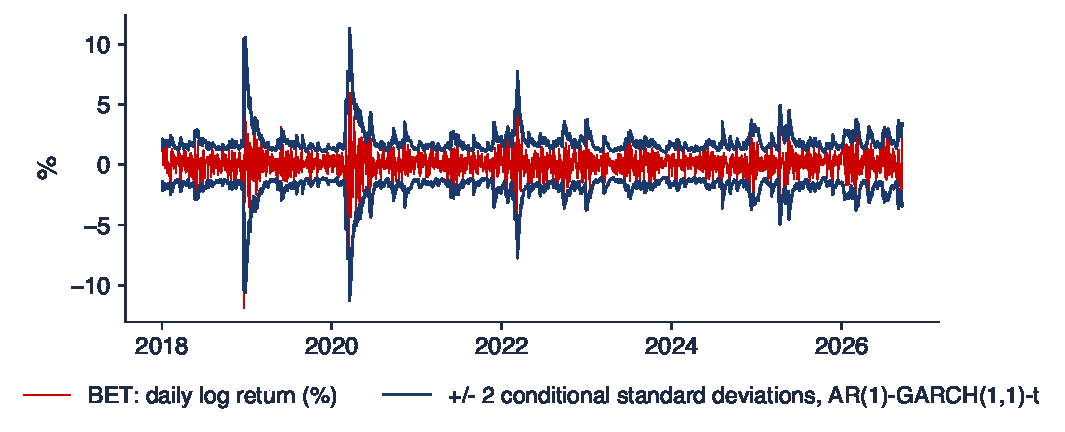
\includegraphics[width=0.96\textwidth,height=0.28\textheight,keepaspectratio]{ch5_sem_b1.pdf}
\end{center}
\vspace{-2mm}
\begin{center}
\scriptsize
\begin{tabular}{lrrrrrr}
\toprule
& $c$ & $\phi$ & $\omega$ & $\alpha$ & $\beta$ & $\nu$ \\
\midrule
estimate & $0.077$ & $0.091$ & $0.0441$ & $0.189$ & $0.801$ & $5.09$ \\
robust SE & $0.010$ & $0.013$ & $0.0085$ & $0.023$ & $0.023$ & $0.32$ \\
\bottomrule
\end{tabular}
\end{center}
\begin{itemize}
    \item AR(1) residuals: ARCH-LM $= nR^2 = 1017$ ($R^2 = 0.153$), $Q(10)$ of squares $= 2496$: strong ARCH effects
    \item $T = 6\,669$; $\alpha + \beta = 0.990$, half-life $\ln 0.5/(-0.01028) = 67.4$ days; long-run volatility 32.8\% against 22.1\% in the sample; $\hat z_t$: $Q(10) = 28.6$ (p $<$\,0.001), $\hat z_t^2$: $7.2$ (p = 0.705)
    \item Peaks: 114\% (2008), 89\% (2020); last day: 26.2\%; 5.1\% of the days fall outside $\pm 2\hat\sigma_t$
    \item Interpretation: below (26.2\% against 32.8\%); the model expects the volatility to rise slowly towards the long-run level, but that level is imprecise ($1 - \alpha - \beta = 0.0102$)
\end{itemize}\quantlet{TSA\_ch5\_seminar}{\qlurl{TSA_ch5_seminar}}
\end{frame}

\begin{frame}{B2: EUR/RON and Bitcoin [Proposed]}
\itemsize{\footnotesize}
\begin{itemize}
\item \textbf{Question}: do the EUR/RON rate and Bitcoin behave like the BET? Model: B1.
\item \textbf{Inputs}: EUR/RON (BNR reference rate) since July 2005, Bitcoin since September 2014; daily log returns in \%
\item \textbf{Tasks}
\begin{enumerate}
    \item Repeat steps 1--4 of B1 for both series (EUR/RON: estimate on $10\,r_t$).
    \item Report $\hat\alpha + \hat\beta$ and say whether the half-life and the long-run volatility exist.
    \item Interpretation: what does $\hat\alpha + \hat\beta = 1$ mean for a forecast of the volatility one year ahead?
\end{enumerate}
\item \textbf{Report}: one table and two sentences
\item Notebook: section B2
\end{itemize}
\end{frame}

\ifsolutions
\begin{frame}{B2: solution [Proposed]}
\itemsize{\footnotesize}
\begin{center}
\scriptsize
\begin{tabular}{lrrrrrrrrr}
\toprule
& $T$ & ARCH-LM & $\phi$ & $\alpha$ & $\beta$ & $\nu$ & $\alpha + \beta$ & sample vol. & $Q(10)$, $\hat z_t^2$ \\
\midrule
EUR/RON & 5\,351 & 811 & $0.031$ & $0.122$ & $0.878$ & $4.21$ & $1.0000$ & 4.4 & $0.004$ \\
Bitcoin & 4\,383 & 106 & $-0.043$ & $0.106$ & $0.894$ & $3.15$ & $1.0000$ & 66.6 & $5.0$ \\
\bottomrule
\end{tabular}
\end{center}
\begin{itemize}
    \item Both: strong ARCH effects before the model; $\hat\alpha + \hat\beta = 1$ (IGARCH): no half-life and no long-run volatility; heavy tails ($\hat\nu$ 4.21 and 3.15)
    \item EUR/RON: $\hat\phi = 0.031$ (OLS: 0.170): the AR term almost disappears once the variance is modelled; $Q(10)$ of $\hat z_t^2$ tiny because of one day (6 May 2025, Lecture 5)
    \item Interpretation: no mean reversion: the forecast for every horizon equals tomorrow's variance, as for EWMA; a one-year forecast simply repeats today's level
\end{itemize}\quantlet{TSA\_ch5\_seminar}{\qlurl{TSA_ch5_seminar}}
\end{frame}
\fi

\begin{frame}{B3: the leverage effect in the S\&P 500 [Solved]}
\itemsize{\footnotesize}
\begin{itemize}
\item \textbf{Question}: do falls raise the volatility of the S\&P 500 more than rises of the same size?
\item \textbf{Inputs}: S\&P 500 closes since 2000, daily log returns in \%
\item \textbf{Tasks}
\begin{enumerate}
    \item Estimate GARCH(1,1)-t and GJR-GARCH(1,1)-t; report $\gamma$ with its robust $t$ statistic.
    \item Compute the LR statistic of GJR against GARCH, its p-value and the two BIC values.
    \item Run the sign-bias test on the standardised residuals of GARCH-t.
    \item Draw both news impact curves and compute the GJR variance after shocks of $-2\%$ and $+2\%$.
    \item Interpretation: how does the leverage effect change the VaR on the day after a fall?
\end{enumerate}
\item \textbf{Report}: four statistics with p-values, two variances, the chart and two sentences
\item Notebook: section B3
\end{itemize}
\end{frame}

\begin{frame}{B3: solution [Solved]}
\itemsize{\scriptsize}
\begin{center}
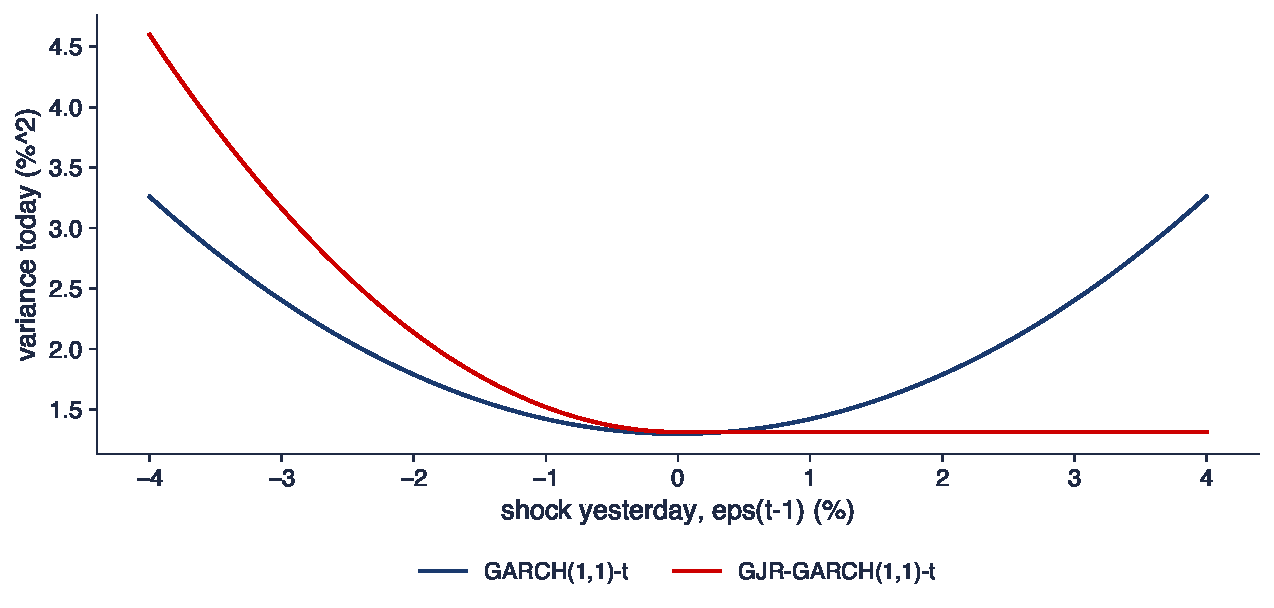
\includegraphics[width=0.96\textwidth,height=0.34\textheight,keepaspectratio]{ch5_sem_b3.pdf}
\end{center}
\vspace{-2mm}
\begin{itemize}
    \item GJR: $\hat\alpha = 0.000$, $\hat\gamma = 0.205$ ($t = 10.0$), $\hat\beta = 0.881$; LR $= 235.7$ (p $<$\,0.001); BIC $18169.0 \to 17942.2$
    \item Sign bias on the GARCH-t residuals: $\chi^2(3) = 40.7$ (p $<$\,0.001), sign $t = 3.56$
    \item GJR variance after $-2\%$: $2.14$; after $+2\%$: $1.31$; ratio $1.62$
    \item Interpretation: only falls raise the variance ($\hat\alpha = 0$); after a fall the VaR is about $\sqrt{1.62} = 1.27$ times the VaR after an equal rise; a symmetric GARCH understates the risk after bad days
\end{itemize}\quantlet{TSA\_ch5\_seminar}{\qlurl{TSA_ch5_seminar}}
\end{frame}

\begin{frame}{B4: asymmetry in the BET, EUR/RON and Bitcoin [Proposed]}
\itemsize{\footnotesize}
\begin{itemize}
\item \textbf{Question}: is there a leverage effect in the BET, in EUR/RON and in Bitcoin? Model: B3.
\item \textbf{Inputs}: BET since 2000, EUR/RON since 2005, Bitcoin since 2014; daily log returns in \%
\item \textbf{Tasks}
\begin{enumerate}
    \item Estimate GJR-GARCH(1,1)-t and EGARCH(1,1)-t; report both values of $\gamma$ with robust $t$ statistics.
    \item Compute the LR test of GJR against GARCH and the change in BIC.
    \item Interpretation: for EUR/RON a positive return means a weaker leu; what is ``bad news'' for this series?
\end{enumerate}
\item \textbf{Report}: one table and two sentences
\item Notebook: section B4
\end{itemize}
\end{frame}

\ifsolutions
\begin{frame}{B4: solution [Proposed]}
\itemsize{\footnotesize}
\begin{center}
\footnotesize
\begin{tabular}{lrrrrrrrr}
\toprule
& GJR $\alpha$ & GJR $\gamma$ & $t$ & LR & p & $\Delta$BIC & EGARCH $\gamma$ & $t$ \\
\midrule
BET & $0.172$ & $0.043$ & ${2.1}$ & $4.9$ & 0.026 & ${3.9}$ & ${-0.028}$ & ${-2.6}$ \\
EUR/RON & $0.103$ & $0.039$ & ${3.0}$ & $9.3$ & 0.002 & ${-0.7}$ & ${-0.040}$ & ${-2.5}$ \\
Bitcoin & $0.113$ & $-0.013$ & ${-0.7}$ & $0.7$ & 0.416 & ${7.7}$ & ${0.015}$ & ${1.2}$ \\
\bottomrule
\end{tabular}
\end{center}
\begin{itemize}
    \item BET: $\gamma > 0$ (EGARCH $\gamma < 0$), significant by LR at 5\%, but BIC rises: a real but small effect
    \item Bitcoin: no asymmetry ($t = -0.7$); EUR/RON: $\gamma > 0$ and significant, with BIC almost unchanged
    \item Interpretation: in GJR the ``bad news'' are $\varepsilon_{t-1} < 0$, days when the leu strengthens; for a currency the sign has no leverage meaning: a large move in either direction signals policy news
\end{itemize}\quantlet{TSA\_ch5\_seminar}{\qlurl{TSA_ch5_seminar}}
\end{frame}
\fi

\begin{frame}{B5: GARCH against EWMA for the S\&P 500 [Solved]}
\itemsize{\footnotesize}
\begin{itemize}
\item \textbf{Question}: does GARCH(1,1)-t forecast tomorrow's variance of the S\&P 500 better than EWMA, and is its VaR 1\% exceeded on 1\% of the days?
\item \textbf{Inputs}: S\&P 500 since 2000; forecasts for every day since 2 January 2015
\item \textbf{Tasks}
\begin{enumerate}
    \item Re-estimate GARCH(1,1)-t every 250 days on all data up to that day and compute the one-day forecasts $h_t$; compute EWMA with $\lambda = 0.94$.
    \item Compute the mean QLIKE of both models and the Diebold--Mariano $t$ statistic.
    \item Count the exceedances of the GARCH-t VaR 1\% and of the EWMA-Normal VaR 1\%, and compare them with the expected number.
    \item Draw the cumulative difference of the losses.
    \item Interpretation: which model would you give to a risk manager, and what would you still improve?
\end{enumerate}
\item \textbf{Report}: four numbers, two counts, the chart and two sentences
\item Notebook: section B5
\end{itemize}
\end{frame}

\begin{frame}{B5: solution [Solved]}
\itemsize{\scriptsize}
\begin{center}
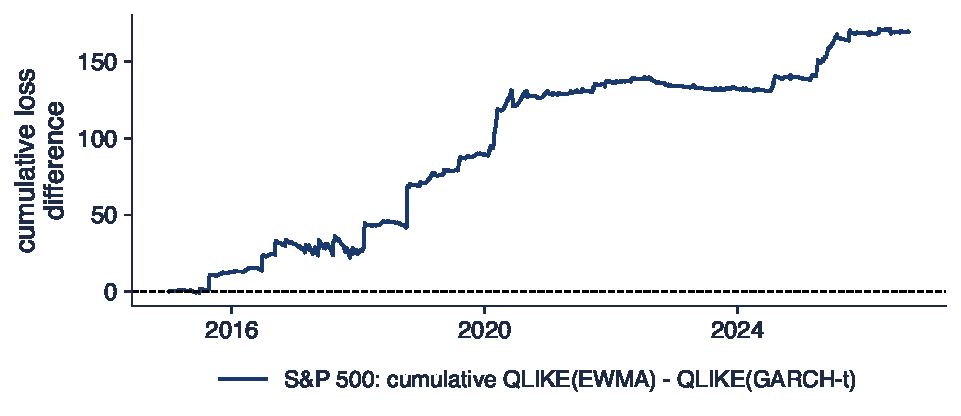
\includegraphics[width=0.96\textwidth,height=0.32\textheight,keepaspectratio]{ch5_sem_b5.pdf}
\end{center}
\vspace{-2mm}
\begin{itemize}
    \item 2\,944 days; mean QLIKE: GARCH-t $0.761$, EWMA $0.819$; DM: mean difference $-0.058$, $t = -3.69$ (p $<$\,0.001): GARCH-t is better
    \item VaR 1\% exceedances: GARCH-t 49 (1.66\%), EWMA-Normal 65 (2.21\%); expected about 29
    \item Interpretation: GARCH-t, but both VaR models are exceeded too often; add the leverage effect (B3) and test the number of exceedances formally (\refKupiec)
\end{itemize}\quantlet{TSA\_ch5\_seminar}{\qlurl{TSA_ch5_seminar}}
\end{frame}

\begin{frame}{B6: GARCH against EWMA for the BET and EUR/RON [Proposed]}
\itemsize{\footnotesize}
\begin{itemize}
\item \textbf{Question}: does the result of B5 hold for the BET and for EUR/RON? Model: B5.
\item \textbf{Inputs}: BET since 2000, EUR/RON since 2005; forecasts for every day since January 2015
\item \textbf{Tasks}
\begin{enumerate}
    \item Compute the out-of-sample GARCH(1,1)-t and EWMA forecasts as in B5.
    \item Compute the mean QLIKE of both models and the DM test.
    \item Find the day with the largest loss difference, and recompute the mean QLIKE without it.
    \item Count the VaR 1\% exceedances of both models.
    \item Interpretation: why can the DM test be insignificant when one mean QLIKE is half the other?
\end{enumerate}
\item \textbf{Report}: one table and two sentences
\item Notebook: section B6
\end{itemize}
\end{frame}

\ifsolutions
\begin{frame}{B6: solution [Proposed]}
\itemsize{\footnotesize}
\begin{center}
\scriptsize
\begin{tabular}{lrrrrrrr}
\toprule
& QLIKE, GARCH-t & EWMA & DM $t$ (p) & largest day & share & exc., GARCH-t & EWMA \\
\midrule
BET & $0.680$ & $0.788$ & ${-2.22}$ (0.027) & 19 December 2018 & 39\% & 34 & 67 \\
EUR/RON & $2.456$ & $5.982$ & ${-1.02}$ (0.310) & 6 May 2025 & 98\% & 35 & 63 \\
\bottomrule
\end{tabular}
\end{center}
\begin{itemize}
    \item Expected VaR 1\% exceedances: about 29 for each series; BET: GARCH-t better (DM $t = -2.22$), exceedances: 34, EWMA-Normal about twice too many
    \item EUR/RON: mean QLIKE 2.456 against 5.982, but DM $t = -1.02$: 98\% of the difference comes from 6 May 2025; without it: $-3.932$ against $-3.877$
    \item Interpretation: the DM statistic divides the mean difference by its standard error; one enormous loss inflates both, so the evidence rests on one day and is weak
\end{itemize}\quantlet{TSA\_ch5\_seminar}{\qlurl{TSA_ch5_seminar}}
\end{frame}
\fi


%=============================================================================
\section{Part C: open questions and AI critique}
%=============================================================================

\begin{frame}{C1: is the leu calmer than it used to be? [Proposed]}
\itemsize{\footnotesize}
\begin{itemize}
\item \textbf{Question}: has the volatility of EUR/RON changed between 2005--2012, 2013--2019 and 2020--2026, and can one GARCH model describe all three periods?
\item \textbf{Inputs}: EUR/RON daily log returns in \% (BNR reference rate); model: B1
\item \textbf{Tasks}
\begin{enumerate}
    \item For each period compute the annualised sample volatility and the share of days with $|r_t| > 0.5\%$.
    \item Estimate GARCH(1,1)-t on each period and report $\alpha + \beta$, $\alpha$ and $\nu$.
    \item Find the largest daily move of each period and its date.
    \item Interpretation: is the change in volatility a property of the market, or of the exchange-rate policy?
\end{enumerate}
\item \textbf{Report}: a table and a plan for a project
\item Notebook: section C1
\end{itemize}
\end{frame}

\ifsolutions
\begin{frame}{C1: reference analysis [Proposed]}
\itemsize{\footnotesize}
\begin{center}
\scriptsize
\begin{tabular}{lrrrrrrr}
\toprule
Period & $T$ & vol.\ (\% p.a.) & $|r| > 0.5\%$ (\%) & $\alpha + \beta$ & $\alpha$ & $\nu$ & max $|r|$ \\
\midrule
2005--2012 & 1\,908 & 6.7 & 15.4 & 1.000 & $0.195$ & $4.53$ & 2.93 \\
2013--2019 & 1\,761 & 3.0 & 2.4 & 1.000 & $0.109$ & $4.14$ & 1.71 \\
2020--2026 & 1\,683 & 1.7 & 0.7 & 1.000 & $0.187$ & $3.45$ & 1.42 \\
\bottomrule
\end{tabular}
\end{center}
\begin{itemize}
    \item Volatility falls from 6.7\% to 3.0\% and 1.7\% per year; large days from 15.4\% to 0.7\% of the days
    \item Every period is IGARCH ($\alpha + \beta = 1$) with very heavy tails: long calm stretches broken by rare jumps (largest moves: 3 October 2008, 7 June 2013, 19 May 2025)
    \item Interpretation: the policy of the BNR, not the market, sets the level; a GARCH with constant parameters fits none of the periods well; project: Markov switching (\tsachlink{https://danpele.github.io/Time-Series-Analysis/EN/Courses/chapter10_state_space_kalman_markov_switching.pdf}{Chapter 10}) or a GARCH with policy dummies
\end{itemize}\quantlet{TSA\_ch5\_seminar}{\qlurl{TSA_ch5_seminar}}
\end{frame}
\fi

\begin{frame}{C2: audit an AI answer [Proposed]}
\itemsize{\scriptsize}
\begin{itemize}
    \item A student asked an AI assistant to interpret a GARCH(1,1)-t fit of the BET (daily, since 2000): $\hat\omega = 0.0448$, $\hat\alpha = 0.192$, $\hat\beta = 0.799$, $\hat\nu = 5.01$. The answer:
    \item \aiprompt{(a) The half-life of a volatility shock is ln 0.5 / ln beta = 3.1 days.}
    \item \aiprompt{(b) The long-run variance is omega/(1 - alpha) = 0.055, an annual volatility of 3.7\%.}
    \item \aiprompt{(c) An AR(1) by OLS gives phi = 0.109 with SE 0.012, t = 8.9: BET returns are strongly predictable.}
    \item \aiprompt{(d) Ljung-Box Q(10) of the squared standardised residuals = 8.3, p = 0.60: the GARCH-t model is correct.}
    \item \aiprompt{(e) With Student-t innovations the 1\% quantile of z is closer to 0 than the Normal -2.326, so the VaR 1\% is smaller.}
    \item \aiprompt{(f) alpha + beta = 0.991 < 1, so the model is covariance stationary and the volatility reverts to its long-run level.}
    \item Tasks
    \begin{itemize}
        \item 1. For each statement, say whether it is correct; if not, give the correct statement and, where possible, the correct number from the notebook (section C2).
        \item 2. Report: a list of six verdicts with one line of justification each.
    \end{itemize}
\end{itemize}
\end{frame}

\ifsolutions
\begin{frame}{C2: solution [Proposed]}
\itemsize{\footnotesize}
\begin{itemize}
    \item (a) Wrong: the half-life uses the persistence, $\ln 0.5/\ln(\alpha + \beta) = \ln 0.5/\ln 0.991 = 74$ days
    \item (b) Wrong: $\bar\sigma^2 = \omega/(1 - \alpha - \beta) = 4.82$, a long-run volatility of 34.7\% (imprecise, since $1 - \alpha - \beta$ is small)
    \item (c) Wrong: with GARCH errors the OLS SE is too small; robust SE 0.029 ($t = 3.8$); AR(1)-GARCH-t: $\hat\phi = 0.091$ ($t = 6.8$); significant, but $\phi^2 \approx 0.012$ of the variance: weak predictability
    \item (d) Wrong: no ARCH effect is left, but that does not prove the model correct; $Q(10)$ of $\hat z_t$ is 114.6: autocorrelation is left in the mean (Lecture 5: AR(1)-GARCH)
    \item (e) Wrong: for the standardised $t$ with $\nu = 5.01$ the quantile is $-2.606$, further from 0 than $-2.326$: the VaR 1\% is larger
    \item (f) Correct
\end{itemize}\quantlet{TSA\_ch5\_seminar}{\qlurl{TSA_ch5_seminar}}
\end{frame}
\fi


%=============================================================================
\section{Wrap-up}
%=============================================================================

\begin{frame}{Key takeaways}
\itemsize{\small}
\begin{itemize}
    \item Test for ARCH effects on the residuals of the mean model: ARCH-LM $= nR^2$ and Ljung--Box on the squares
    \item $\alpha + \beta$ decides the long run: half-life, long-run variance, the shape of the forecasts; $\alpha + \beta = 1$: IGARCH
    \item Multi-day risk is the sum of the daily variance forecasts, not $\sqrt{H}$ times today's volatility
    \item Heavy-tailed innovations change the VaR quantile; asymmetry changes the VaR after bad days
    \item Compare forecasts out of sample (QLIKE, DM) and look for single days that drive the result
\end{itemize}
\end{frame}

\begin{frame}{After the seminar}
\itemsize{\small}
\begin{itemize}
    \item Lecture 5 develops each topic of today: stylised facts, ARCH and GARCH, estimation, ARMA-GARCH, asymmetry, diagnostics, forecasts, VaR 1\%
    \item Try the [Proposed] tasks in the notebook
    \item C1 can grow into a team project: volatility regimes of the leu and of other currencies of the region
    \item Reading: \refHP, Ch.~6; \refTsay, Ch.~3
    \item \textbf{The seminar is for practice and is not graded; the solutions of [Proposed] tasks are discussed in class}
\end{itemize}
\end{frame}


%=============================================================================
\section{References}
%=============================================================================

\begin{frame}{References}
\itemsize{\tiny}
\begin{itemize}
    \item Bollerslev, T. (1986). Generalized autoregressive conditional heteroskedasticity. \textit{Journal of Econometrics}, 31(3), 307--327. \href{https://doi.org/10.1016/0304-4076(86)90063-1}{doi:10.1016/0304-4076(86)90063-1}
    \item Bollerslev, T. (1987). A conditionally heteroskedastic time series model for speculative prices and rates of return. \textit{Review of Economics and Statistics}, 69(3), 542--547. \href{https://doi.org/10.2307/1925546}{doi:10.2307/1925546}
    \item Bollerslev, T., \& Wooldridge, J. M. (1992). Quasi-maximum likelihood estimation and inference in dynamic models with time-varying covariances. \textit{Econometric Reviews}, 11(2), 143--172. \href{https://doi.org/10.1080/07474939208800229}{doi:10.1080/07474939208800229}
    \item Christie, A. A. (1982). The stochastic behavior of common stock variances: Value, leverage and interest rate effects. \textit{Journal of Financial Economics}, 10(4), 407--432. \href{https://doi.org/10.1016/0304-405X(82)90018-6}{doi:10.1016/0304-405X(82)90018-6}
    \item Diebold, F. X., \& Mariano, R. S. (1995). Comparing predictive accuracy. \textit{Journal of Business \& Economic Statistics}, 13(3), 253--263. \href{https://doi.org/10.1080/07350015.1995.10524599}{doi:10.1080/07350015.1995.10524599}
    \item Engle, R. F. (1982). Autoregressive conditional heteroscedasticity with estimates of the variance of United Kingdom inflation. \textit{Econometrica}, 50(4), 987--1007. \href{https://doi.org/10.2307/1912773}{doi:10.2307/1912773}
    \item Engle, R. F., \& Ng, V. K. (1993). Measuring and testing the impact of news on volatility. \textit{Journal of Finance}, 48(5), 1749--1778. \href{https://doi.org/10.1111/j.1540-6261.1993.tb05127.x}{doi:10.1111/j.1540-6261.1993.tb05127.x}
    \item Glosten, L. R., Jagannathan, R., \& Runkle, D. E. (1993). On the relation between the expected value and the volatility of the nominal excess return on stocks. \textit{Journal of Finance}, 48(5), 1779--1801. \href{https://doi.org/10.1111/j.1540-6261.1993.tb05128.x}{doi:10.1111/j.1540-6261.1993.tb05128.x}
    \item Huang, C., \& Petukhina, A. (2022). \textit{Applied Time Series Analysis and Forecasting with Python}. Springer. \href{https://doi.org/10.1007/978-3-031-13584-2}{doi:10.1007/978-3-031-13584-2}
    \item J.P. Morgan/Reuters (1996). \textit{RiskMetrics -- Technical Document} (4th ed.). Morgan Guaranty Trust Company. \href{https://www.msci.com/documents/10199/5915b101-4206-4ba0-aee2-3449d5c7e95a}{msci.com}
    \item Kupiec, P. H. (1995). Techniques for verifying the accuracy of risk measurement models. \textit{Journal of Derivatives}, 3(2), 73--84. \href{https://doi.org/10.3905/jod.1995.407942}{doi:10.3905/jod.1995.407942}
    \item Ljung, G. M., \& Box, G. E. P. (1978). On a measure of lack of fit in time series models. \textit{Biometrika}, 65(2), 297--303. \href{https://doi.org/10.1093/biomet/65.2.297}{doi:10.1093/biomet/65.2.297}
    \item Nelson, D. B. (1991). Conditional heteroskedasticity in asset returns: A new approach. \textit{Econometrica}, 59(2), 347--370. \href{https://doi.org/10.2307/2938260}{doi:10.2307/2938260}
    \item Patton, A. J. (2011). Volatility forecast comparison using imperfect volatility proxies. \textit{Journal of Econometrics}, 160(1), 246--256. \href{https://doi.org/10.1016/j.jeconom.2010.03.034}{doi:10.1016/j.jeconom.2010.03.034}
    \item Tsay, R. S. (2010). \textit{Analysis of Financial Time Series} (3rd ed.). Wiley. \href{https://doi.org/10.1002/9780470644560}{doi:10.1002/9780470644560}
\end{itemize}
\end{frame}

\end{document}
